\documentclass[14pt]{extreport}

\usepackage[utf8]{inputenc}
\usepackage[T2A]{fontenc}
\usepackage[english,ukrainian]{babel}
\usepackage{tempora}

\usepackage{float}
\usepackage{caption}
\captionsetup[table]{justification=raggedleft, singlelinecheck=false, labelsep=space}
\captionsetup[figure]{labelsep=space}
\usepackage{graphicx}
\graphicspath{ {./pictures} }

\usepackage{longtable}
\usepackage{multirow}
\usepackage{ragged2e}
\usepackage{array}
\newcolumntype{C}[1]{>{\Centering\arraybackslash}m{#1\textwidth}}
\newcolumntype{L}[1]{>{\raggedright\arraybackslash}m{#1\textwidth}}
\addto\captionsukrainian{
  \renewcommand{\tablename}{Таблиця}
}
\newenvironment{tight}{
  \begingroup
  \linespread{1.15}\selectfont
}{
  \endgroup
}

\linespread{1.5}
\setlength{\parskip}{0pt}
\usepackage{indentfirst}

\usepackage[a4paper,top=20mm,bottom=20mm,left=25mm,right=10mm]{geometry}

\usepackage{fancyhdr}
\fancypagestyle{plain}{
  \pagestyle{myheadings}
}
\pagestyle{myheadings}
\setcounter{page}{4}

\setcounter{secnumdepth}{3}
\newcounter{req}[subsubsection]
\newcommand\req{\arabic{req}\stepcounter{req}}

\usepackage{titlesec}
\titleformat{\chapter}{\centering\bfseries\MakeUppercase}{\chaptername~\thechapter.}{1pc}{}
\titleformat{\section}{\bfseries}{\thesection.}{1pc}{}
\titleformat{\subsection}{\bfseries}{\thesubsection.}{1pc}{}
\titleformat{\subsubsection}{\bfseries}{\thesubsubsection.}{1pc}{}
% \titleformat{\paragraph}{\bfseries}{}{}{}

\titlespacing*{\chapter}{0pt}{10mm}{14pt}
\titlespacing*{\section}{\parindent}{14pt}{0pt}
\titlespacing*{\subsection}{\parindent}{0pt}{0pt}
\titlespacing*{\subsubsection}{\parindent}{0pt}{0pt}
\titlespacing*{\paragraph}{\parindent}{0pt}{7pt}

\usepackage{enumitem}
\setlist{nolistsep}

\usepackage{hyperref}
\def\UrlBreaks{\do\/\do-}

\usepackage[acronym, nonumberlist]{glossaries}
\makeglossaries
\renewcommand{\glossarysection}[2][]{}
\newacronym{pow}{PoW}{Proof of Work}
\newacronym{pos}{PoS}{Proof of Stake}
\newacronym{poh}{PoH}{Proof of History}
\newacronym{dpos}{DPoS}{Delegated Proof of Stake}
\newacronym{pbft}{PBFT}{Practical Byzantine Fault Tolerance}
\newacronym{poa}{PoA}{Proof of Authority}
\newacronym{poet}{PoET}{Proof of Elapsed Time}
\newacronym{pospace}{PoSpace}{Proof of Space}
\newacronym{poc}{PoC}{Proof of Capacity}
\newacronym{p2p}{P2P}{Peer-to-Peer}
\newacronym{tps}{TPS}{транзакції на секунду}
\newacronym{rpc}{RPC}{Remote Procedure Call}
\newacronym{sdk}{SDK}{Software Development Kit}
\newacronym{bft}{BFT}{Byzantine Fault Tolerance}
\newacronym{http}{HTTP}{Hypertext Transfer Protocol}
\newacronym{https}{HTTPS}{Hypertext Transfer Protocol Secure}
\newacronym{pda}{PDA}{Program Derived Address}

\newcommand{\plainchap}[1]{
  \chapter*{#1}
}
\newcommand{\tocchap}[1]{
  \chapter*{#1}
  \addcontentsline{toc}{chapter}{\MakeUppercase{#1}}
}
\newcommand{\tocnumchap}[1]{
  \refstepcounter{chapter}
  \chapter*{\MakeUppercase{\chaptername}~\thechapter.\hspace{1em}\MakeUppercase{#1}}
  \addcontentsline{toc}{chapter}{\MakeUppercase{\chaptername}~\thechapter.\hspace{1em}\MakeUppercase{#1}}
}

\usepackage{listings}
\usepackage{multicol}
\usepackage{courier}
\renewcommand{\ttdefault}{pcr}
\lstset{
  basicstyle=\ttfamily,
	tabsize=2,
	keepspaces,
	showstringspaces=false,
	breaklines,
}

\begin{document}
  \plainchap{Анотація}
  
  \tableofcontents
  \newpage

  \tocchap{Перелік скорочень, символів і спеціальних термінів}
  
  \printglossaries
  
  \tocchap{Вступ}
  
  У сучасному світі цифрові технології відіграють ключову роль у забезпеченні прозорості, достовірності та довіри в різних сферах суспільного життя. Однією з таких сфер є електронне голосування — інноваційний підхід до організації виборів, який дедалі частіше використовується як альтернатива традиційним паперовим методам. Електронне голосування дозволяє зменшити витрати часу та ресурсів, підвищити зручність участі, а також розширити коло учасників. Однак широке впровадження таких систем стикається з рядом викликів, серед яких — забезпечення цілісності даних, запобігання фальсифікаціям, гарантування конфіденційності виборців, а також підтвердження легітимності результатів.

  Сучасні централізовані електронні системи голосування залишаються вразливими до низки загроз, включно з технічними збоями, зовнішніми атаками, внутрішніми маніпуляціями та недовірою з боку користувачів. Відсутність повної прозорості процесу створює передумови для спотворення результатів, що у свою чергу знижує рівень довіри суспільства до інституцій, які організовують такі голосування. Одним із перспективних напрямів розв'язання цих проблем є використання технології блокчейн. Блокчейн знаходить застосування в багатьох галузях, включаючи фінанси, логістику, охорону здоров'я та управління ланцюгами поставок. У контексті електронного голосування він дозволяє забезпечити прозорість, конфіденційність і захищеність голосів: кожен голос у такій системі зберігається у вигляді транзакції, яка є незмінною та відкритою для перевірки всіма учасниками. Завдяки цьому досягається високий рівень довіри до процесу голосування навіть без централізованого контролю.

  Актуальність теми цієї роботи зумовлена потребою у створенні сучасних електронних систем голосування, які забезпечуватимуть високий рівень безпеки та довіри. З розвитком технологій все більше організацій, компаній та державних установ прагнуть впроваджувати цифрові рішення для голосування, що потребує детального аналізу існуючих підходів, а також розробки нових моделей, що враховуватимуть їх переваги та недоліки.

  Метою роботи є проєктування системи для проведення голосувань та опитувань, яка відповідатиме вимогам прозорості, безпеки та достовірності результатів. Для забезпечення поставленої мети розроблено архітектуру системи голосування, яка відповідає вимогам безпеки, надійності та ефективності.

  Для досягнення поставленої мети необхідно виконати низку задач, зокрема провести комплексне дослідження існуючих рішень у сфері електронного голосування, зосередивши увагу на системах, побудованих із використанням технології блокчейн. На основі цього слід визначити ключові переваги та недоліки таких рішень і сформулювати вимоги до безпечної, прозорої та зручної у використанні платформи для голосування. Далі потрібно спроєктувати архітектуру майбутньої системи, що передбачає механізми створення голосувань, автентифікації користувачів, захисту даних і прозорої обробки результатів. Після цього необхідно реалізувати основні компоненти системи та провести тестування з метою перевірки її функціональності, стабільності роботи й відповідності визначеним вимогам безпеки.

  Результати цієї роботи можуть бути використані для подальшого розвитку електронних систем голосування, а також як основа для впровадження подібних рішень у різних сферах діяльності — від державного управління до корпоративних голосувань та соціальних опитувань.
  
  % Оглядовий розділ
  \tocnumchap{Теоретичні основи та аналіз сучасних підходів до організації електронних голосувань}
  
  \section{Основи блокчейн-технології}

  Блокчейн є децентралізованою технологією зберігання даних, яка дозволяє створювати надійні розподілені системи без потреби в довіреному централізованому органі. Основною її особливістю є здатність забезпечувати незмінність і прозорість інформації завдяки використанню криптографічних методів та особливої структури зберігання. На рис~\ref{fig:blockchain} зображено загальну структуру блокчейну, що ілюструє зв’язки між блоками, їхній вміст та хеш-значення попередніх блоків \cite{blockchain_structure}.

  \begin{figure}[H]
    \centering
    \includegraphics[scale=3.3]{BlockchainStructure}
    \caption{Схема структури блокчейну}
    \label{fig:blockchain}
  \end{figure}

  Кожен блок у блокчейні містить перелік транзакцій, хеш попереднього блоку та часову позначку \cite{blockchain}. Транзакції в мережі спочатку накопичуються, після чого об'єднуються в блоки — це дозволяє підвищити ефективність обробки та масштабованість системи. Блоки пов'язані між собою у послідовний ланцюг. Якщо змінити хоча б одну транзакцію в блоці, це призведе до зміни його хеша, порушить цілісність усього ланцюга й така спроба буде одразу виявлена. Завдяки цьому блокчейн є стійким до фальсифікацій і несанкціонованого втручання.

  Функціонування блокчейну забезпечується одноранговою \gls{p2p} мережею, в якій кожен вузол має власну копію ланцюга і з'єднаний безпосередньо з іншими учасниками. Вузли взаємодіють між собою, обмінюючись інформацією про транзакції та нові блоки, синхронізуючи свої копії ланцюга. Така архітектура усуває потребу в центральному сервері, забезпечуючи стійкість до збоїв, а також підвищуючи надійність і прозорість системи: усі транзакції доступні для перегляду кожному учаснику, що дозволяє перевіряти достовірність інформації без довіри до окремого адміністратора.

  Таким чином, децентралізація, прозорість і незмінність — це основні риси блокчейн-систем, які роблять їх надійним фундаментом для побудови цифрових інфраструктур, включно з фінансовими платформами, ланцюгами постачання та електронним голосуванням.

  \section{Методи досягнення консенсусу у розподілених системах}

  Однією з ключових складових технології блокчейн є механізм досягнення консенсусу, необхідний для узгодження єдиного порядку транзакцій та додавання нових блоків у децентралізовану мережу. У розподілених системах, де дані зберігаються та обробляються незалежними вузлами без центрального органу управління, виникає ризик розбіжностей між учасниками через одночасне надходження кількох транзакцій або через можливість недобросовісної поведінки окремих вузлів. Без механізму консенсусу система може стати вразливою до атак або втратити свою цілісність, оскільки вузли не зможуть дійти згоди щодо єдиного стану ланцюжка блоків. Ефективний механізм консенсусу вирішує ці проблеми, забезпечуючи синхронізацію дій вузлів, незмінність даних та довіру між учасниками мережі \cite{consensus}.

  Один із найпоширеніших алгоритмів консенсусу — \gls{pow}, або доказ виконаної роботи \cite{pow}. У цьому алгоритмі вузли мережі змагаються за право додати новий блок до ланцюжка, розв'язуючи складну криптографічну задачу. Перший вузол, який успішно знаходить розв'язок, отримує винагороду, а його блок додається до ланцюжка. \gls{pow} забезпечує безпеку системи завдяки високій обчислювальній складності, проте має значні недоліки, включаючи високе енергоспоживання та обмежену масштабованість.

  Інший популярний алгоритм — \gls{pos}, або доказ частки володіння \cite{pos}. У цьому підході вузол, що додає новий блок, обирається пропорційно до кількості криптовалюти, яку він утримує. \gls{pos} значно знижує енергоспоживання порівняно з \gls{pow} та забезпечує вищу продуктивність, проте може викликати занепокоєння щодо концентрації влади у власників великої кількості криптовалюти.

  Серед сучасних альтернативних підходів виділяється \gls{poh} \cite{poh}. \gls{poh} впроваджує механізм впорядкування подій у часі за допомогою криптографічних міток часу. Це дозволяє вузлам мережі перевіряти порядок транзакцій незалежно від інших вузлів, що значно підвищує швидкість обробки даних і забезпечує високу пропускну здатність. \gls{poh} унікальний тим, що додає часовий компонент до процесу консенсусу, що знижує необхідність тривалих узгоджень між вузлами.

  \begin{table}[H]
  \caption{\\\centering\textbf{Порівняння алгоритмів консенсусу}}
  \label{tab:consensus_comparison}
  \resizebox{\textwidth}{!}{
    \begin{tabular}{|C{0.3}|C{0.2}|C{0.2}|C{0.2}|}
    \hline
    \textbf{Критерій} & \textbf{PoW} & \textbf{PoS} & \textbf{PoH} \\ \hline
    \textbf{Безпека} & Висока & Висока & Висока \\ \hline
    \textbf{Енергоспоживання} & Високе & Низьке & Низьке \\ \hline
    \textbf{Масштабованість} & Низька & Середня & Висока \\ \hline
    \textbf{Швидкість} & Низька & Середня & Висока \\ \hline
    \end{tabular}
  }
  \end{table}
  
  Таким чином, різні алгоритми консенсусу забезпечують баланс між безпекою, продуктивністю та енергоспоживанням. Вибір конкретного механізму залежить від особливостей застосування блокчейну. У контексті електронного голосування важливими факторами є швидкість обробки транзакцій, масштабованість, низькі витрати та захищеність, що впливає на вибір найбільш відповідного алгоритму для створення ефективної системи. З огляду на це, для реалізації системи електронного голосування найбільш доцільним є використання алгоритму \gls{poh}. На відміну від \gls{pow} і \gls{pos}, \gls{poh} забезпечує високу швидкість обробки транзакцій, високу масштабованість та низьке енергоспоживання завдяки вбудованому часовому компоненту, який дозволяє вузлам незалежно та швидко верифікувати порядок подій. Це зменшує затримки при досягненні консенсусу та є критично важливим для забезпечення швидкодії та доступності системи.
  
  Окрім основних методів консенсусу, існують інші підходи, як-от \gls{dpos}, де делегати обираються для прийняття рішень; \gls{pbft}, який застосовується в приватних блокчейнах для забезпечення консенсусу при наявності шахраїв; \gls{poa}, де валідатори обираються на основі їх авторитету; \gls{poet}, який використовує випадковий час очікування для визначення лідера блоку; \gls{pospace} і \gls{poc}, що залучають вільне місце на диску для досягнення консенсусу з меншими енергетичними витратами. Проте ці алгоритми не набули широкого використання, оскільки використовуються переважно в специфічних умовах.
  
  \section{Інноваційні підходи у технологіях електронного голосування}
  
    Електронне голосування є одним із ключових напрямів цифровізації суспільства, який дозволяє підвищити зручність та доступність виборчих процесів. Традиційні електронні системи, хоч і широко використовуються, стикаються з численними викликами, зокрема щодо забезпечення прозорості, безпеки та захищеності від маніпуляцій. Сучасні інноваційні підходи у цій сфері спрямовані на вирішення цих проблем за рахунок використання новітніх технологій.

  Одним із таких підходів є застосування блокчейн-технології, яка забезпечує децентралізоване зберігання даних і гарантує незмінність записів. У системах голосування на основі блокчейну кожен голос реєструється як транзакція, яка зберігається у ланцюжку блоків. Це дозволяє кожному учаснику перевірити правильність підрахунку голосів, зберігаючи при цьому конфіденційність виборців. Крім того, блокчейн унеможливлює зміну результатів голосування без відома більшості учасників, що підвищує рівень довіри до системи.

  Іншим важливим напрямом є використання криптографічних методів для забезпечення безпеки та анонімності виборців. Зокрема, технології шифрування даних і цифрового підпису дозволяють гарантувати, що голос може бути зарахований лише від авторизованого виборця, а його зміст залишається недоступним для третіх сторін. Ці методи також забезпечують захист від дублювання голосів або спроб втручання у виборчий процес.

  Застосування інноваційних підходів дозволяє вирішити ключові проблеми, притаманні традиційним електронним системам голосування. Проте впровадження цих технологій вимагає подолання ряду викликів, таких як висока вартість розробки, необхідність адаптації до юридичних норм та забезпечення масштабованості системи. Незважаючи на ці труднощі, інноваційні рішення відкривають нові можливості для створення прозорих, безпечних та доступних виборчих процесів.
  
  \section{Огляд та аналіз існуючих рішень для організації голосувань}

  Системи голосування постійно еволюціонують, охоплюючи як традиційні офлайн та онлайн централізовані моделі, так і новітні децентралізовані рішення. Вибір підходу залежить від цілей, масштабу, вимог до безпеки та ступеня довіри між учасниками процесу.

  Одним із найпоширеніших підходів є централізовані офлайн-системи голосування, які використовуються на виборчих дільницях. Вони базуються на спеціалізованому апаратному та програмному забезпеченні (електронні урни, сканери бюлетенів), контрольованому єдиним оператором або групою довірених органів. Такі системи забезпечують високу швидкість обробки голосів і зручність для виборчих комісій. Проте вони мають суттєві недоліки: обмежена прозорість для виборців, потреба в повній довірі до адміністратора системи, ризики технічних збоїв або втручання в ланцюг постачання обладнання.

  Іншим різновидом є централізовані онлайн-системи голосування, які забезпечують дистанційну участь виборців через інтернет. Вони реалізуються як веб- або мобільні застосунки і особливо корисні в умовах пандемій чи для виборців за кордоном. Попри зручність, ці системи мають свої виклики: захист від кібератак, гарантія цілісності та конфіденційності голосів, запобігання повторному голосуванню, а також складність незалежної верифікації результатів.
  
  У зв’язку з викликами, притаманними централізованим рішенням, зростає зацікавленість у децентралізованих системах голосування, зокрема на основі блокчейн-технологій. У таких системах дані про голоси зберігаються в розподіленому реєстрі, змінити який без консенсусу учасників мережі практично неможливо. Платформи на кшталт Voatz декларують використання блокчейну для досягнення прозорості, незмінності та довіри \cite{voatz}. Водночас Voatz критикували за закритість вихідного коду та виявлені вразливості \cite{voatzcriticism}, що підкреслює важливість відкритості й незалежного аудиту в таких рішеннях.

  Ще одним прикладом масштабного впровадження електронного голосування є система i-Voting в Естонії \cite{ivoting}, яка з 2017 року дає громадянам змогу голосувати онлайн із використанням електронного підпису. Хоча ця система не базується на блокчейні, вона спирається на перевірену інфраструктуру електронної ідентифікації та шифрування й продемонструвала на практиці свою ефективність у загальнодержавному масштабі.
  
  Для кращого розуміння відмінностей між централізованими та децентралізованими підходами у сфері електронного голосування, у таблиці~\ref{tab:voting_systems_comparison} наведено порівняння ключових характеристик обох типів систем за основними критеріями, що впливають на їхню ефективність, надійність та придатність до практичного використання. Оскільки існують різні реалізації блокчейнів, кожен з яких має свої характеристики, показники децентралізованих систем можуть суттєво варіюватися в залежності від вибраної платформи.
  
  \begin{table}[H]
    \caption{\\\centering\textbf{Порівняння централізованих та децентралізованих систем голосування}}
    \label{tab:voting_systems_comparison}
    \resizebox{\textwidth}{!}{
      \begin{tabular}{|C{0.3}|C{0.35}|C{0.35}|}
      \hline
      \textbf{Критерій} & \textbf{Централізовані системи} & \textbf{Децентралізовані системи} \\ \hline
      \textbf{Прозорість} & Низька & Висока \\ \hline
      \textbf{Безпека} & Середня & Висока \\ \hline
      \textbf{Масштабованість} & Висока & Залежить від реалізації \\ \hline
      \textbf{Енергоспоживання} & Низьке & Залежить від реалізації \\ \hline
      \textbf{Швидкість} & Висока & Залежить від реалізації \\ \hline
      \end{tabular}
    }
  \end{table}
  
  Аналіз демонструє, що централізовані рішення переважають у зрілості та практичності, проте обмежені в прозорості та довірі. Натомість децентралізовані рішення пропонують привабливу альтернативу, що вимагає вирішення проблем масштабованості, складності впровадження, зручності для користувачів та юридичного регулювання \cite{ieee:almeida}. Зважаючи на ці фактори, дослідження в напрямку побудови блокчейн-орієнтованих систем електронного голосування є актуальним і перспективним.
  
  \section{Висновки до розділу}
  
  У цьому розділі було розглянуто основні аспекти технології блокчейн, методи досягнення консенсусу у розподілених системах, інноваційні підходи до електронного голосування та існуючі рішення для організації виборчих процесів. Аналіз існуючих рішень продемонстрував, що децентралізовані платформи на основі блокчейн-технології мають значний потенціал для вирішення ключових проблем електронного голосування. Подальший розвиток цих технологій, спрямований на подолання технічних і організаційних бар'єрів, дозволить створити прозорі, безпечні та доступні системи голосування, які відповідають сучасним вимогам.
  
  % Розділ постановки завдання
  \tocnumchap{Постановка завдання розроблення застосунку та обґрунтування вибору технологій}

  \section{Мета та завдання розробки}
  
  Метою роботи є створення функціональної та надійної системи електронного голосування, яка забезпечить підвищення прозорості, безпеки та довіри до процесу волевиявлення шляхом застосування технології блокчейн. Розроблена система має вирішити існуючі проблеми централізованих рішень, зокрема залежність від операторів, потенційний ризик маніпуляцій з даними голосування та необхідність забезпечення високого рівня безпеки.

  Для досягнення поставленої мети необхідно виконати наступні завдання:
  
  \begin{enumerate}
    \item Розробити деталізовану архітектуру системи електронного голосування, визначивши ключові модулі, їхню взаємодію та відповідальність. Архітектурне рішення має враховувати вимоги до безпеки, масштабованості та зручності використання.
    \item Реалізувати програмну частину системи, включаючи смарт-контракти на блокчейн-платформі, а також клієнтський вебінтерфейс для взаємодії користувачів із системою.
    \item Забезпечити інтеграцію з криптовалютним гаманцем для безпечної аутентифікації користувачів та підписання транзакцій голосування.
    \item Створити та провести тестування розробленої системи на відповідність визначеним функціональним та нефункціональним вимогам, включаючи перевірку безпеки, продуктивності та зручності використання.
    \item Підготувати технічну документацію, що описує процес розробки, архітектуру системи, інструкції з використання та результати тестування.
  \end{enumerate}
  
  \section{Характеристика об'єкту проєктування}
  
  Об'єктом проєктування є децентралізована система електронного голосування, що функціонує на основі блокчейн-технології.
  
  Вхідними даними для розробленого програмного забезпечення є:
  
  \begin{itemize}
    \item Реєстраційна інформація користувачів (ідентифікатори, публічні ключі гаманців), що отримується з підключеного гаманця. Формат представлення – дані, що передаються через вебформи та API гаманця.
    \item Параметри голосування, що задаються організатором через вебінтерфейс (назва, опис, перелік варіантів вибору, тривалість голосування). Формат представлення – структуровані дані, що передаються через вебформи.
    \item Подані голоси користувачів, що вибираються ними через вебінтерфейс та підписуються за допомогою їхніх приватних ключів. Формат представлення – ідентифікатор обраного варіанту та криптографічний підпис транзакції.
  \end{itemize}
  
  Вихідними даними розробленого програмного забезпечення є:
  
  \begin{itemize}
    \item Захищені та незмінні записи про проведені голосування та подані голоси, що зберігаються у блокчейні. Формат представлення – транзакції та дані у відповідних облікових записах блокчейну.
    \item Результати голосування, що агрегуються на основі даних з блокчейну та відображаються користувачам через вебінтерфейс у текстовому та графічному форматах.
    \item Сповіщення про статус голосу (успішно подано, помилка), що відображаються користувачам у вебінтерфейсі. Формат представлення – текстові повідомлення та візуальні елементи інтерфейсу.
  \end{itemize}
  
  \section{Обґрунтування вибору технологій та методів}
  
  Як видно з таблиці~\ref{tab:voting_systems_comparison}, децентралізовані системи голосування мають значні переваги порівняно з централізованими, зокрема високу прозорість та безпеку. Саме тому для розробки системи обрано блокчейн як технологічну основу. Однак для ефективного використання цих переваг необхідно обрати блокчейн-платформу, яка забезпечує високу масштабованість, низьке енергоспоживання та швидкість обробки транзакцій. Саме тому для реалізації системи було обрано платформу Solana, яка завдяки інноваційному механізму консенсусу \gls{poh} демонструє високу продуктивність і стабільну роботу навіть за великого навантаження, що є критично важливим для системи голосування з великою кількістю учасників. Solana здатна обробляти до 65,000 \gls{tps} \cite{solana_report}, що значно перевищує показники багатьох інших блокчейн-платформ.

  Мову програмування для розробки смарт-контрактів було обрано Rust. Однією з основних причин вибору Rust є його висока продуктивність та безпека. Rust дозволяє контролювати управління пам'яттю без використання збирача сміття, що дозволяє досягати кращої ефективності та передбачуваності в порівнянні з іншими мовами. Мова забезпечує гарантії безпеки пам'яті через систему власності і запозичення, що дозволяє уникати багатьох типових помилок, таких як витоки пам'яті або доступ до неініціалізованої пам'яті, зберігаючи високу продуктивність. Такий підхід є особливо важливим при розробці смарт-контрактів для блокчейн-платформи, де потрібно обробляти великі обсяги транзакцій і зберігати ефективність виконання програм при обмежених ресурсах. Завдяки цьому Rust є ідеальним вибором для розробки смарт-контрактів на Solana.

  Для спрощення процесу розробки смарт-контрактів на Solana було обрано використання бібліотеки Anchor. Anchor - це фреймворк для розробки смарт-контрактів, який забезпечує більш високий рівень абстракції і значно спрощує роботу з Solana, дозволяючи швидше і безпечніше створювати смарт-контракти. Anchor також допомагає в автоматизації багатьох аспектів розробки, таких як перевірка транзакцій, підписання і виконання, що дозволяє зосередитися на бізнес-логіці, а не на низькорівневих деталях взаємодії з блокчейном.

  % TODO: any other will do
  Важливою частиною застосунку є інтеграція з криптовалютним гаманцем для забезпечення безпечного доступу користувачів до системи. Вибір Phantom Wallet зумовлений не лише його популярністю серед користувачів Solana, а й зручністю для розробників. Phantom надає простий інтерфейс для взаємодії зі смарт-контрактами, що значно спрощує інтеграцію з блокчейном і пришвидшує розробку. Він також підтримує безпечне зберігання ключів і легке підтвердження транзакцій, що робить його оптимальним вибором для системи голосування.

  Для клієнтської частини застосунку обрано React, що дозволяє створювати зручні та інтерактивні вебзастосунки. Завдяки своїй популярності і широкій підтримці бібліотек, React забезпечує гнучкість і масштабованість, необхідні для розробки інтерфейсу користувача для системи голосувань.
  
  \section{Аналіз вимог}
  
  На етапі аналізу вимог було проведено ретельне дослідження предметної області електронного голосування. Це дозволило визначити ключові потреби основних зацікавлених сторін: організаторів голосувань та учасників (виборців). Метою аналізу було формування чіткого переліку функціональних та нефункціональних вимог до розроблюваної системи, які стали підґрунтям для подальшої детальної специфікації.
  
  Організатори голосувань мають потребу у зручному інструменті для створення та гнучкого налаштування голосувань, включаючи визначення назви, опису, варіантів вибору та терміну дії. Вони також зацікавлені у можливості контролювати процес голосування та, за необхідності (з урахуванням анонімності), переглядати проміжну статистику. Ключовою вимогою є забезпечення прозорості та незмінності результатів для зміцнення довіри до процесу волевиявлення, а також надання простого способу оголошення підсумків після завершення голосування. У перспективі, за потреби, можлива інтеграція системи з іншими платформами або системами обліку користувачів.
  
  Учасники голосувань мають потребу в інтуїтивно зрозумілому інтерфейсі для зручної участі в голосуваннях. Для них критично важливим є забезпечення анонімності їхнього волевиявлення та захист від розкриття зробленого вибору. Виборці також зацікавлені у можливості ознайомлення з результатами голосування після його завершення. Безпека системи та неможливість фальсифікації результатів є для них першочерговими вимогами, так само як і зручний спосіб ідентифікації та автентифікації для участі у голосуванні.
  
  \section{Специфікація вимог}
  
  Призначенням застосунку є забезпечення прозорого, безпечного та незмінного процесу голосування завдяки використанню технології блокчейну. Він дозволяє організаторам ініціювати голосування, визначати варіанти вибору та переглядати результати, а учасникам безпечно віддавати свої голоси.
  
  % \subsubsection{Продукти-аналоги} 
  
  \subsection{Загальний опис}
  \subsubsection{Характеристики продукту} 
  
  Розроблена система електронного голосування надає наступні основні можливості:
  
  \begin{itemize}
    \item Організатори можуть ініціювати голосування, визначаючи назву, опис, перелік варіантів вибору та термін дії.
    \item Зареєстровані учасники можуть безпечно віддавати свої голоси за один із запропонованих варіантів протягом визначеного терміну.
    \item Після завершення голосування всі користувачі можуть переглядати підсумки голосування у наочному форматі.
  \end{itemize}
  
  \subsubsection{Класи користувачів та їх характеристики}
  Користувачі системи поділяються на два класи:
  \begin{itemize}
    \item Організатор голосування – користувач, який має право створювати, налаштовувати та контролювати параметри голосування (назва, опис, варіанти, час завершення). Організатор також може брати участь у створеному ним голосуванні як звичайний виборець.
    \item Учасник голосування (виборець) – користувач, який має право брати участь в активних голосуваннях, віддаючи свій голос за один із варіантів. Для участі виборець повинен мати встановлений та налаштований криптовалютний гаманець. 
  \end{itemize}
  
  Як організатори, так і учасники голосування є пріоритетним класом користувачів, оскільки без їхньої взаємодії функціонування системи є неможливим.
  
  \subsubsection{Середовище функціонування}
  Програмний продукт функціонує у децентралізованому середовищі блокчейну Solana. Смарт-контракти, що реалізують основну логіку голосування, виконуються в мережі Solana. Клієнтська частина системи розроблена як вебзастосунок, що працює у сучасних браузерах та взаємодіє зі смарт-контрактами через \gls{rpc}-сервіси Solana. Для взаємодії з користувачами використовується криптовалютний гаманець.

  \subsection{Характеристики системи}
  \subsubsection{Створення голосування}  
  \paragraph{Опис:} Організатор може створювати голосування з заданими параметрами.  
  \paragraph{Пріоритет:} Високий.
  \paragraph{Послідовність дія/відгук:}  
  \begin{enumerate}  
      \item Організатор входить у застосунок.  
      \item Вибирає опцію створення голосування.  
      \item Вводить параметри голосування (назва, опис, варіанти, час до завершення).  
      \item Підтверджує створення голосування.  
      \item Система перевіряє дані та публікує голосування у блокчейні.  
      \item Система повідомляє організатора про успішне створення.  
  \end{enumerate}
  \paragraph{Функціональні вимоги:}
  \begin{itemize}[leftmargin=*,label=REQ-\arabic{subsubsection}.\req:]  
      \item Система має забезпечувати форму для параметрів голосування.
      \item Система перевіряє коректність введених даних.
      \item Система інтегрується зі смарт-контрактом для запису даних у блокчейн.  
  \end{itemize}

  \subsubsection{Участь у голосуванні}  
  \paragraph{Опис:} Виборець може подати свій голос за один із варіантів голосування.  
  \paragraph{Пріоритет:} Високий.  
  \paragraph{Послідовність дія/відгук:}  
  \begin{enumerate}  
      \item Виборець входить у систему.  
      \item Вибирає активне голосування.  
      \item Обирає варіант голосування.  
      \item Підтверджує вибір.  
      \item Система перевіряє валідність голосу (уникнення повторного голосування).  
      \item Система записує голос у блокчейн.  
      \item Виборець отримує підтвердження успішного голосування.  
  \end{enumerate}  
  \paragraph{Функціональні вимоги:}  
  \begin{itemize}[leftmargin=*,label=REQ-\arabic{subsubsection}.\req:]  
      \item Система має дозволяти вибір варіанту голосування.  
      \item Система перевіряє валідність голосу перед його подачею.  
      \item Система записує голос через смарт-контракт у блокчейн.  
  \end{itemize}  

  \subsubsection{Перегляд результатів голосування}  
  \paragraph{Опис:} Учасники можуть переглядати результати після завершення голосування.  
  \paragraph{Пріоритет:} Середній.  
  \paragraph{Послідовність дія/відгук:}  
  \begin{enumerate}  
      \item Користувач входить у систему.  
      \item Вибирає завершене голосування.  
      \item Вибирає опцію перегляду результатів.  
      \item Система зчитує дані з блокчейну.  
      \item Відображає результати голосування у графічному вигляді.  
  \end{enumerate}  
  \paragraph{Функціональні вимоги:}  
  \begin{itemize}[leftmargin=*,label=REQ-\arabic{subsubsection}.\req:]  
      \item Система має дозволяти доступ до завершених голосувань.  
      \item Система інтегрується зі смарт-контрактом для отримання даних.  
      \item Система візуалізує результати у зручному форматі.
  \end{itemize}  

  \subsection{Вимоги зовнішніх інтерфейсів}
  \subsubsection{Користувацькі інтерфейси}
  Користувач взаємодіє із системою через вебінтерфейс, що включає:
  \begin{itemize}
    \item Екран створення голосування (форма з введенням параметрів голосування).
    \item Екран участі у голосуванні (вибір варіанта і підтвердження).
    \item Екран перегляду результатів (графічна візуалізація результатів голосування).
    \item Екран авторизації за допомогою Phantom Wallet для підтвердження особи користувача перед участю у голосуванні.
    \item Екран вибору кластеру мережі Solana.
    \item Екран управління акаунтом у мережі Solana.
  \end{itemize}
  
  \subsubsection{Програмні інтерфейси}
  Система взаємодіє з наступними програмними компонентами:
  \begin{itemize}
    \item Блокчейн Solana — через \gls{rpc}-сервіси для запису та зчитування даних смарт-контрактів.
    \item Криптовалютний гаманець Phantom Wallet — через його API для аутентифікації користувачів та підписання транзакцій.
    \item Браузери (сучасні версії Chrome, Firefox, Safari, Edge, тощо).
    \item Бібліотека Anchor для спрощення взаємодії зі смарт-контрактами Solana.
    \item Бібліотека React для розробки клієнтського вебінтерфейсу.
  \end{itemize}
  
  \subsubsection{Комунікаційні інтерфейси}
  Вебзастосунок використовує стандартні протоколи \gls{http}, \gls{https} для взаємодії з \gls{rpc}-сервісами Solana. Для взаємодії з гаманцем Phantom Wallet використовуються специфічні методи, передбачені його API. Безпека комунікацій забезпечується використанням протоколу \gls{https}.
  
  \subsection{Інші нефункційні вимоги}
  \subsubsection{Вимоги продуктивності}
  \begin{itemize}
    \item Час підтвердження голосу не повинен перевищувати 3 секунд (Не враховуючи час на взаємодію з гаманцем Phantom Wallet).
    \item Час відображення результатів голосування не повинен перевищувати 5 секунд.  
    \item Система повинна підтримувати одночасну участь 1000 користувачів без значного зниження продуктивності (час відгуку на дії користувача не повинен збільшуватися більше ніж на 20%).
  \end{itemize}

  \subsubsection{Вимоги безпеки}
  \begin{itemize}
    \item Доступ до функціональності створення та редагування голосувань повинен бути обмежений лише авторизованими організаторами.
    \item Система повинна гарантувати, що кожен користувач може проголосувати лише один раз в межах одного голосування.
    \item Голоси, подані користувачами, повинні бути перевірені на валідність перед записом у блокчейн.
  \end{itemize}
  
  \subsubsection{Атрибути якості програмного продукту}
  \begin{itemize}  
    \item Кодова база повинна мати модульну та читабельну структуру для полегшення подальшої розробки, тестування та підтримки.
    \item Система повинна бути стійкою до тимчасових втрат з'єднання з блокчейном та автоматично відновлювати свою роботу після відновлення з'єднання.
    \item Основна функціональність системи повинна бути покрита автоматизованими тестами (юніт-тести, інтеграційні тести) для забезпечення відповідності вимогам та виявлення потенційних помилок.
    \item Інтерфейс користувача повинен бути інтуїтивно зрозумілим та зручним у використанні для користувачів з різним рівнем технічної підготовки.
  \end{itemize}

  % \subsection{Інші вимоги}
 
  \section{Висновки до розділу}
  
  У цьому розділі було сформульовано мету та завдання розробки, а також обґрунтовано вибір технологій, алгоритмів і інструментів, які використовуються для реалізації системи голосування. Проаналізовано вимоги до системи, включаючи функціональні та нефункціональні аспекти, що дозволило визначити ключові параметри, необхідні для забезпечення її надійності, безпеки та зручності використання та сформувати специфікацію вимог.

  % Проєктний розділ
  \tocnumchap{Проєктування децентралізованого застосунку для проведення голосувань}

  \section{Проєктування загальної архітектури застосунку}
  
  Архітектура застосунку для проведення голосувань базується на принципах децентралізації, прозорості та безпеки, що є фундаментальними вимогами для сучасних електронних систем голосування. Застосунок складається з чотирьох основних компонентів: клієнтської частини, гаманця Phantom Wallet, смарт-контракту та блокчейн-платформи Solana. Кожен з них виконує окремі функції у процесі голосування, забезпечуючи ефективну, безпечну та прозору взаємодію між користувачем і блокчейном. Схематичне відображення взаємодії між компонентами представлено на діаграмі компонентів на рисунку~\ref{fig:UMLComponent}.

  \begin{figure}[H]
    \centering
    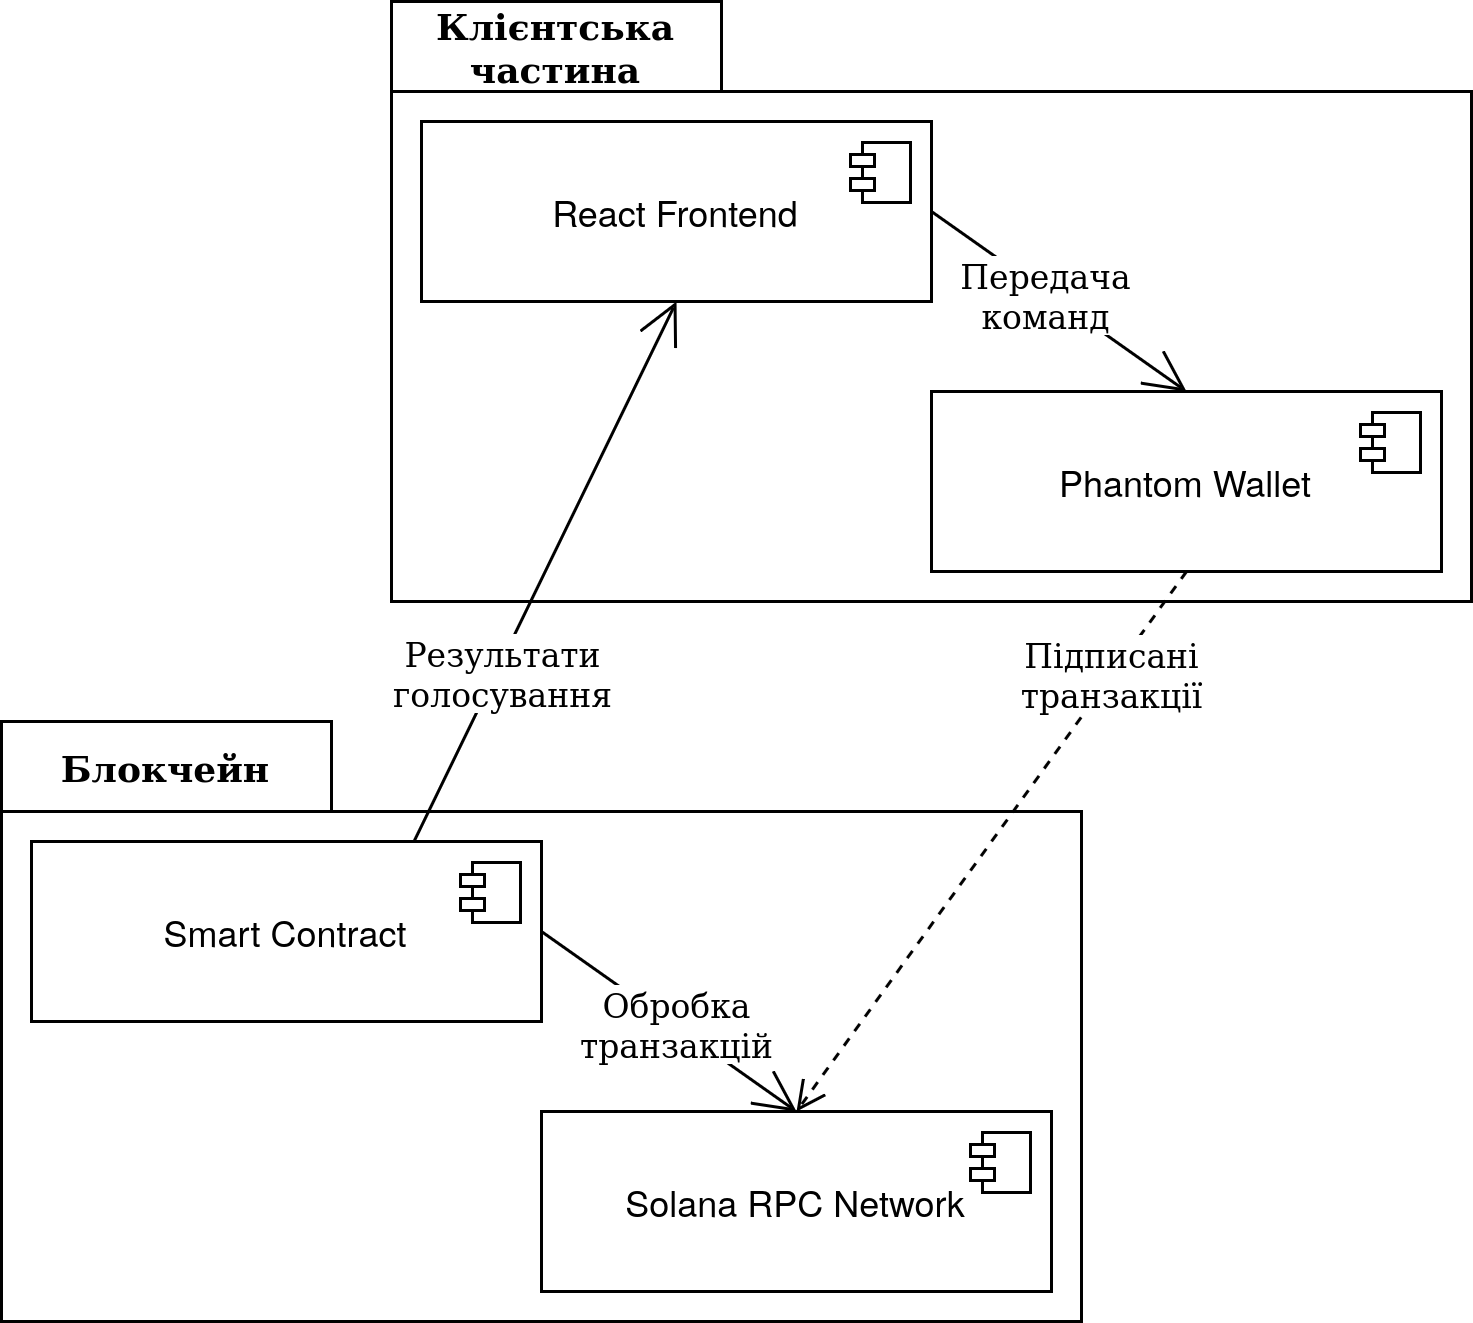
\includegraphics[scale=0.24]{UMLComponent}
    \caption{Діаграма компонентів}
    \label{fig:UMLComponent}
  \end{figure}

  Клієнт є основним інтерфейсом взаємодії користувача із системою. Реалізована за допомогою фреймворку React, вона забезпечує доступ до функціоналу як для організаторів, так і для учасників голосування. Організатори можуть створювати нові голосування, встановлювати варіанти відповідей і визначати дедлайни. Учасники мають змогу переглядати доступні голосування, обирати варіанти та відстежувати результати. Кожна дія користувача (створення голосування, голосування, перегляд результатів) ініціює транзакцію, яка формується у клієнті, підписується через Phantom Wallet та надсилається до смарт-контракту. Таким чином, клієнт виступає посередником між користувачем і блокчейн-інфраструктурою, забезпечуючи зручність та безпеку взаємодії.

  Phantom Wallet — це браузерне розширення, яке забезпечує безпечне зберігання приватних ключів користувача та підпис транзакцій. Його використання є критично важливим для автентифікації та авторизації дій у системі. Під час голосування або створення нового голосування клієнтська частина формує транзакцію, яку користувач повинен підписати своїм приватним ключем через Phantom Wallet. Це гарантує, що жодна дія не може бути виконана від імені користувача без його згоди. Гаманець також забезпечує взаємодію з мережею Solana, виступаючи у ролі шлюзу між користувачем і блокчейном.

  Смарт-контракт є логічним ядром системи голосування, розгорнутим у мережі Solana. Він реалізує повний життєвий цикл голосування: створення опитування, реєстрацію голосів, перевірку права голосу, виключення можливості повторного голосування, підрахунок голосів та збереження результатів. Смарт-контракт є детермінованим і не залежить від зовнішніх сервісів, що гарантує чесність та прозорість виконання логіки. Всі записи зберігаються безпосередньо в блокчейні, що унеможливлює їх зміну або видалення. Це забезпечує довіру до системи і дозволяє будь-кому перевірити достовірність результатів голосування.

  У системі голосування блокчейн Solana виконує роль середовища для зберігання та обробки транзакцій. Кожна дія користувача — створення голосування, голос чи перегляд результатів — перетворюється на транзакцію, яка надсилається до мережі Solana. Ці транзакції перевіряються, обробляються та фіксуються у блокчейні, що гарантує їхню незмінність і публічну доступність. Solana забезпечує високу швидкість обробки та масштабованість, що дозволяє системі працювати ефективно навіть при великій кількості користувачів.

  Узгоджена взаємодія клієнта, гаманця Phantom, смарт-контракту та блокчейну Solana формує цілісну архітектуру, що забезпечує безпечний, прозорий і незмінний процес голосування. Такий підхід дозволяє реалізувати децентралізовану систему, якій можуть довіряти всі учасники, незалежно від їх ролі, забезпечуючи високий рівень надійності та масштабованості.
  
  \section{Проєктування функціональних модулів клієнтської частини}
  
  Функціональність клієнтської частини застосунку організована навколо шести ключових модулів, які забезпечують повний цикл взаємодії користувачів із системою електронного голосування, починаючи від перегляду інформації про власний обліковий запис до безпосередньої участі у голосуваннях та ознайомлення з їхніми результатами. Ці модулі побудовані таким чином, щоб забезпечити інтуїтивно зрозумілий процес для різних категорій користувачів, використовуючи при цьому можливості блокчейн-платформи Solana для гарантування безпеки та прозорості. Взаємодія між користувачами різних ролей та функціональними можливостями системи наочно представлена на діаграмі прецедентів, відображеній на рисунку~\ref{fig:UMLUseCase}.

Діаграма прецедентів ілюструє, як дві основні ролі користувачів – "Виборець" та "Організатор" – взаємодіють із застосунком. "Виборець" має можливість переглядати інформацію про свій обліковий запис, включаючи баланс та історію транзакцій, обирати кластер мережі Solana для роботи, переглядати результати вже завершених голосувань, додавати власну адресу кластеру та, що є його основною функцією, брати участь у голосуваннях шляхом вибору одного з доступних варіантів. Процес голосування є складною дією, яка включає попередній вибір варіанту.

Роль "Організатор" об'єднує в собі всі можливості "Виборця" та додає ключову функцію створення нових голосувань. Цей процес передбачає введення необхідних даних, таких як назва голосування, опис, перелік варіантів вибору та тривалість. Таким чином, діаграма прецедентів демонструє розподіл функціональних можливостей між різними ролями користувачів, підкреслюючи основні сценарії використання системи електронного голосування.

  \begin{figure}[H]
    \centering
    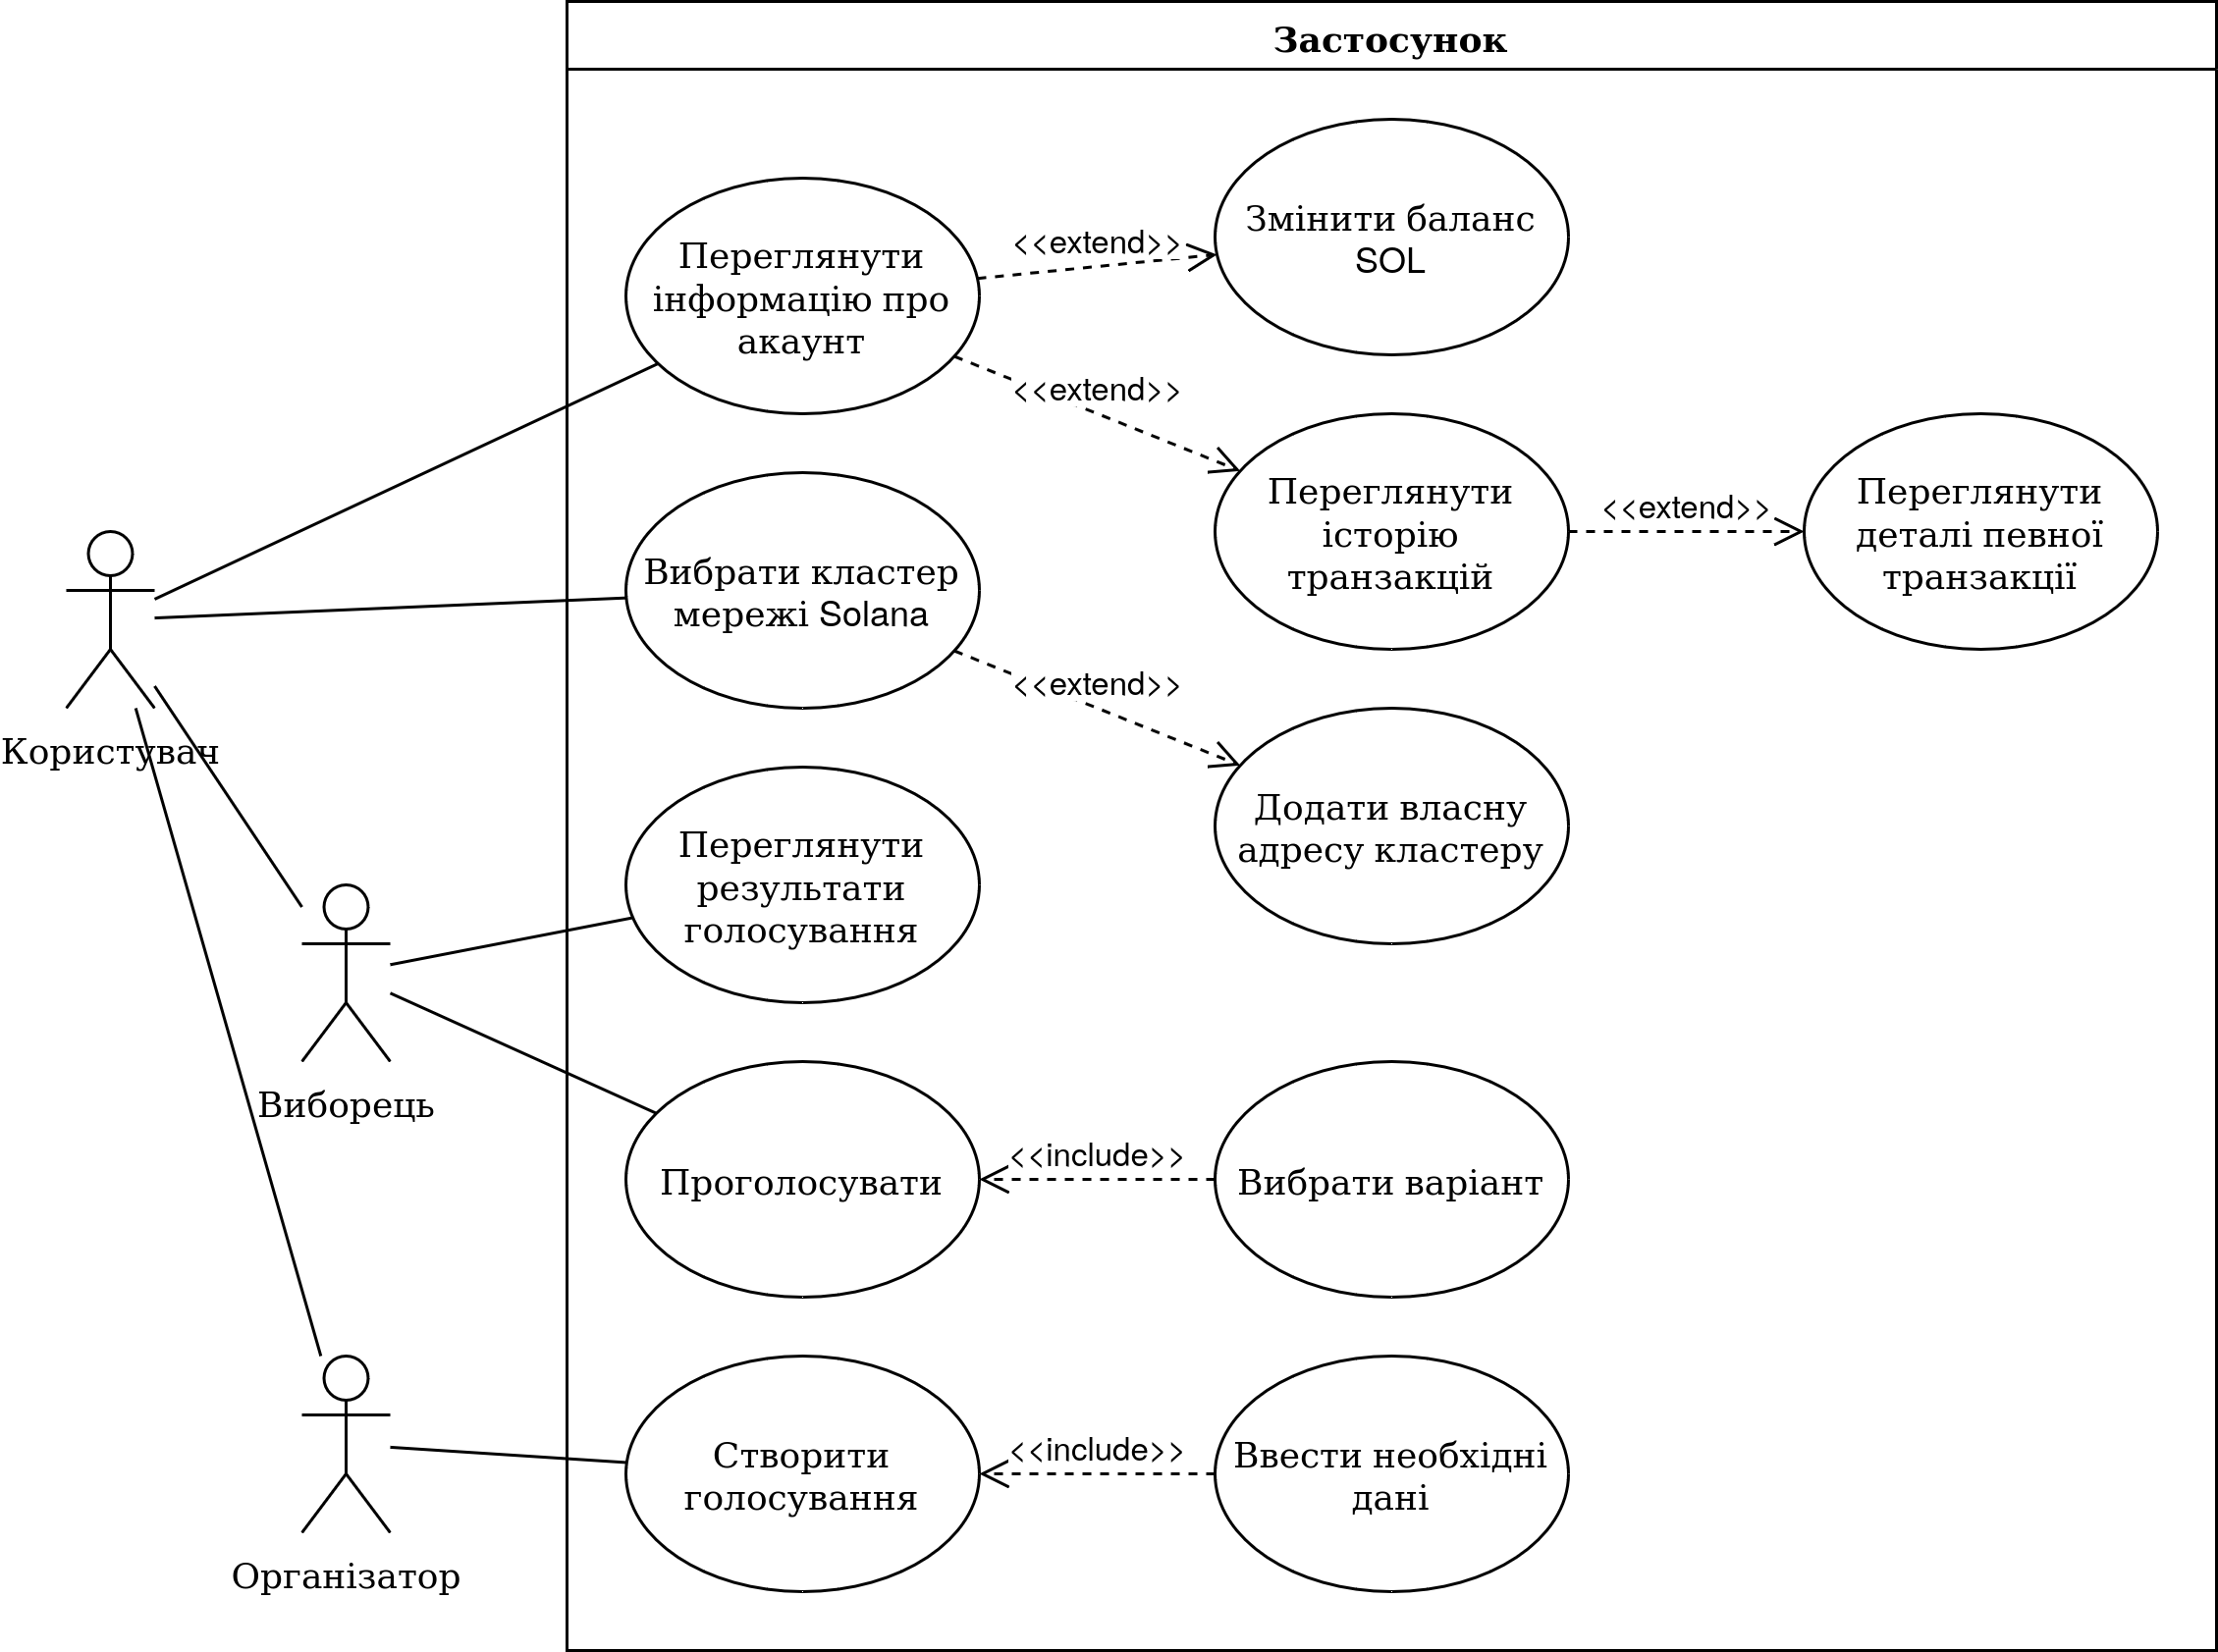
\includegraphics[scale=0.18]{UMLUseCase}
    \caption{Діаграма прецедентів}
    \label{fig:UMLUseCase}
  \end{figure}
  
  \section{Проєктування інтерфейсу користувача та його елементів}
  
  Інтерфейс клієнтської частини застосунку розроблено з фокусом на зручність та інтуїтивність використання, щоб забезпечити ефективну взаємодію користувачів на всіх етапах роботи з системою електронного голосування.

  На рисунку~\ref{fig:UIPolls} зображено головну сторінку застосунку, де відображаються доступні голосування. У верхній частині сторінки розміщено заголовок, та кнопки для вибору між управлінням акаунтом, вибором кластеру та застосунком для голосувань. Нижче розташована коротка інструкція користувача для створення голосування та інформація про обліковий запис користувача, зокрема його ідентифікатор, що підкреслює важливість автентифікації у системі голосування. Центральне місце займає кнопка створення, яка є ключовим елементом для ініціювання процесу створення нового голосування організатором. Важливою частиною цієї сторінки є список доступних голосувань, представлених за їхніми назвами. Користувачі можуть переглядати цей список, щоб знаходити потрібні їм голосування. При натисканні на назву конкретного голосування відкривається діалогове вікно, що відображає детальну інформацію про це голосування та надає можливість взяти в ньому участь. Дизайн сторінки мінімалістичний, з акцентом на простоті та функціональності, щоб користувачі могли легко орієнтуватися та швидко знаходити потрібні опції.

  На рисунку~\ref{fig:UICreate} представлено форму для створення нового голосування. Для того, щоб потрапити на цю сторінку, користувач повинен натиснути кнопку "Create Poll" на головній сторінці застосунку. У верхній частині форми розташовані поля для введення назви голосування та його опису, що дозволяє організатору надати контекст та інформацію про предмет голосування. Нижче знаходиться поле для визначення тривалості голосування, де організатор вказує час, протягом якого голосування буде активним. Тривалість голосування може бути вказана у хвилинах, годинах та днях, що забезпечує гнучкість у плануванні голосування. Далі розташовані поля для введення кандидатів або варіантів вибору та кнопка для додавання нових варіантів. У нижній частині форми знаходяться дві кнопки: для підтвердження створення голосування та для закриття форми. Дизайн форми інтуїтивно зрозумілий, з чіткими підписами до полів введення, що полегшує процес заповнення.

  На рисунку~\ref{fig:UIVote} зображено форму, призначену для подачі голосу учасником голосування. У верхній частині форми відображається назва та опис голосування. Нижче розміщено таймер, який спливає в реальному часі та показує час, що залишився до завершення голосування, що створює відчуття терміновості та стимулює учасників до активності. Після завершення таймера проголосувати більше не можна. Далі представлені варіанти голосування з інформацією про кількість поданих голосів за кожен варіант. Праворуч від кожного варіанту розташована кнопка для подачі голосу. У нижній частині форми знаходиться кнопка для закриття форми. Якщо голосування переглядає організатор, йому також доступна кнопка для зміни параметрів голосування, а саме можливість збільшення тривалості часу до завершення. Дизайн форми зосереджений на простоті та зручності використання, з чітким відображенням варіантів вибору та таймером, що дозволяє учасникам швидко і легко зробити свій вибір.

  На рисунку~\ref{fig:UIResults} представлено вікно з результатами голосування. У верхній частині вікна розміщений заголовок, який одразу інформує користувача про призначення цього екрана. Нижче наведено варіанти відповідей. Для кожного варіанту відображається кількість отриманих голосів та їхній відсоток від загальної кількості. Візуально кількість голосів представлена горизонтальними смугами, довжина яких пропорційна кількості відданих голосів, що полегшує швидке порівняння результатів. Під результатами голосування підсумовується загальна кількість поданих голосів та вказано лідера голосування. У нижній частині вікна розміщено кнопку, яка дозволяє користувачеві закрити вікно з результатами та повернутися до попереднього екрана. Дизайн цього вікна лаконічний та інформативний, основний акцент зроблено на чіткому відображенні результатів голосування.

  На рисунку~\ref{fig:UIClusters} відображено інтерфейс для управління кластерами Solana. У верхній частині сторінки знаходиться заголовок та коротка інструкція користувача, що пояснює призначення сторінки – управління та вибір кластерів Solana. Нижче розташована кнопка, що дозволяє користувачам додавати нові кластери. Основну частину сторінки займає таблиця з переліком доступних кластерів, де для кожного кластера відображаються його назва, мережа та кінцева точка. Кластери Solana – це різні мережі, на яких розгортаються та функціонують програми Solana. Дизайн сторінки структурований, з використанням таблиці для зручного представлення інформації про кластери.

  На рисунку~\ref{fig:UIAccount} представлено інтерфейс, що відображає інформацію про обліковий запис користувача. У верхній частині сторінки розташовані основні функції, пов'язані з управлінням обліковим записом, такі як отримання та передача криптовалюти. Нижче знаходиться інформація про історію транзакцій. Список транзакцій дозволяє користувачам відстежувати всі операції, здійснені з їхнім обліковим записом. Деталі кожної транзакції, такі як хеш, час, статус, можна переглянути на сторонньому сервісі (наприклад, Solana Explorer), що забезпечує прозорість та можливість перевірки операцій. Дизайн сторінки функціональний, з чітким розділенням інформації на блоки.
    
  Таким чином, представлені візуалізації ключових екранів клієнтської частини застосунку демонструють інтуїтивно зрозумілий та функціональний дизайн. Кожен інтерфейс спроєктовано з урахуванням потреб користувачів на різних етапах роботи із системою голосування: від створення опитування та участі в ньому до перегляду результатів та управління власним обліковим записом і вибором кластерів Solana. Простота навігації, чітке представлення інформації та логічне розташування елементів керування сприяють зручній та ефективній взаємодії користувача з застосунком.
  
  \section{Проєктування смарт-контракту}
  
  Смарт-контракт являє собою самовиконуваний код, що зберігається в блокчейні та автоматично виконує умови, прописані в ньому. У контексті цього застосунку, смарт-контракт відповідає за створення опитувань, реєстрацію голосів та забезпечення чесності процесу голосування. Інструкція в смарт-контракті – це дія, яку користувач може ініціювати для взаємодії з контрактом. Кожна інструкція виконує певну функцію, наприклад, створення нового опитування або подача голосу. Транзакція – це підписане повідомлення, яке користувач надсилає в мережу блокчейн для виконання певної інструкції смарт-контракту. Транзакція включає в себе дані інструкції та підпис користувача, що підтверджує його автентичність.
  
  У блокчейні Solana для зберігання даних використовується акаунти. Існують два основних типи акаунтів: акаунти, що належать системній програмі, які використовуються для базових операцій, таких як переказ коштів або виділення місця для даних, та акаунти, що належать програмам, які використовуються для зберігання стану смарт-контрактів та пов'язаних з ними даних.
  
  Для функціонування смарт-контракту застосунку для проведення голосувань необхідні наступні акаунти:
  
  \begin{itemize}
    \item Акаунт підписувача – це акаунт користувача, який ініціює транзакцію. Він потрібен для оплати комісій за транзакції та підписання інструкцій.
    \item Акаунт опитування – зберігає інформацію про конкретне опитування, включаючи його назву, опис, час завершення, список кандидатів та кількість голосів за кожного кандидата. Оскільки кожне опитування є унікальним, для кожного нового опитування створюється окремий акаунт опитування.
    \item Акаунт виборця – відіграє ключову роль у запобіганні повторному голосуванню. Коли користувач вперше голосує в певному опитуванні, для нього створюється унікальний акаунт виборця, пов'язаний як з самим опитуванням, так і з публічним ключем користувача. Коли той самий користувач спробує проголосувати в цьому ж опитуванні вдруге, смарт-контракт перевірить, чи існує акаунт виборця, пов'язаний з його публічним ключем та цим опитуванням. Якщо такий акаунт вже існує, це означає, що користувач вже віддав свій голос, і транзакція на голосування буде відхилена.
  \end{itemize}
  
  Архітектурно, смарт-контракт розроблений таким чином, щоб забезпечити чітке розділення між логікою створення опитування та логікою голосування. Взаємодія з блокчейном відбувається через надсилання підписаних транзакцій. Клієнт створює транзакцію, яка містить необхідну інструкцію та дані, підписує її своїм приватним ключем і надсилає в мережу Solana. Мережа верифікує підпис та виконує інструкцію смарт-контракту, оновлюючи стан відповідних акаунтів.

  Для створення опитування клієнт ініціює транзакцію, яка викликає інструкцію у смарт-контракті. У цій транзакції клієнт передає назву опитування, його опис, час завершення та список кандидатів. Смарт-контракт перевіряє ці дані на валідність та створює новий акаунт опитування, зберігаючи в ньому передану інформацію. Адреса цього акаунта опитування детерміновано генерується на основі назви опитування, що дозволяє унікально ідентифікувати кожне опитування.

  Для голосування клієнт ініціює транзакцію, яка викликає інструкцію vote у смарт-контракті. У цій транзакції клієнт передає назву опитування та ім'я кандидата, за якого він хоче проголосувати. Смарт-контракт перевіряє, чи існує опитування з такою назвою, чи не закінчився час голосування, чи існує кандидат з вказаним ім'ям, і чи не голосував вже даний користувач у цьому опитуванні (перевіряючи наявність відповідного акаунта виборця). Якщо всі перевірки проходять успішно, смарт-контракт збільшує лічильник голосів для обраного кандидата в акаунті опитування та створює або оновлює акаунт виборця, фіксуючи факт голосування цього користувача в даному опитуванні.
  
  Смарт-контракт, у свою чергу, зберігає в блокчейні стан опитувань (назва, опис, час завершення, кандидати, кількість голосів) та інформацію про те, хто і в якому опитуванні вже проголосував. Усі ці дані є публічними та незмінними після запису в блокчейн, що забезпечує прозорість та чесність процесу голосування.
  
  Схематично роботу смарт-контракту зображено на діаграмі послідовності на рисунку~\ref{fig:UMLSequence},
  
  \begin{figure}[H]
    \centering
    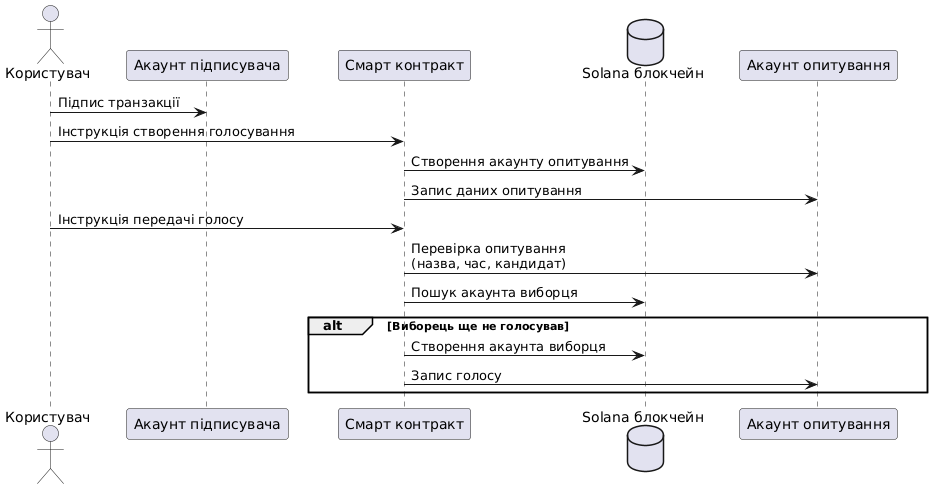
\includegraphics[scale=0.5]{UMLSequence}
    \caption{Діаграма послідовності}
    \label{fig:UMLSequence}
  \end{figure}
  
  \section{Проєктування безпеки та конфіденційності}
  
  Забезпечення безпеки та конфіденційності є фундаментальним елементом архітектури застосунку для голосувань, оскільки саме ці аспекти формують базову довіру користувачів до легітимності та незворотності результатів. У рамках розробки системи було впроваджено багатошарову модель захисту, яка використовує передові методи криптографії, протоколи шифрування та алгоритмічні механізми валідації даних.

  Для унеможливлення повторного голосування застосовується система валідації унікальності транзакцій. Кожен голос супроводжується унікальним криптографічним маркером, що генерується на основі комбінації відкритого ключа користувача, даних про голосування та випадкового доповнення. Смарт-контракт на рівні Solana Runtime Environment аналізує ці маркери і здійснює детерміновану валідацію автентичності кожного голосу у режимі реального часу.

  Щодо перевірки валідності голосу, перед його зарахуванням виконується перевірка підпису транзакції приватним ключем користувача. Додатково, перед надсиланням транзакції у мережу, відбувається локальна верифікація за допомогою Phantom Wallet \gls{sdk}, що гарантує збереження приватного ключа у зашифрованому середовищі пристрою користувача без жодної можливості його витоку в мережу.

  Анонімність учасників забезпечується шляхом використання псевдонімізації, де кожному користувачеві призначається унікальний криптографічний ідентифікатор. Ідентифікатор створюється на основі випадково згенерованого ентропійного значення та додаткових криптографічних операцій, що не дозволяють встановити зв'язок із особистими даними користувача. Відповідність голосу певному ідентифікатору перевіряється без розкриття особистості голосуючого, що забезпечує приватність даних у процесі голосування.
  
  Блокчейн-технологія забезпечує високий рівень захисту від кібератак та маніпуляцій з даними завдяки своїм властивостям. Після того як голос зареєстрований у блокчейні, його неможливо змінити або видалити. Це забезпечується завдяки структурі блокчейну, що гарантує незмінність і стійкість до маніпуляцій завдяки криптографічному зв'язку блоків через унікальні хеші. Кожна зміна будь-якого елемента даних миттєво призводить до розриву зв'язності у мережі, що робить підробку практично неможливою без повного контролю над переважною більшістю вузлів (чого досягти надзвичайно складно через географічну та інституційну децентралізацію мережі).
  
  Крім того, блокчейн Solana застосовує унікальну модель консенсусу \gls{poh} у комбінації з Tower \gls{bft} - гібридний механізм, що забезпечує високу пропускну здатність транзакцій без зниження безпеки. \gls{poh} синхронізує події у часовій шкалі за допомогою криптографічних часових міток, що унеможливлює атаки типу "подвійного витрачання" навіть при високих навантаженнях на мережу. Ця властивість дозволяє системі підтримувати мілісекундні затримки обробки та мільйонні обсяги транзакцій на годину.
  
  \section{Висновки до розділу}
  
  У цьому розділі було розглянуто архітектуру децентралізованого застосунку для проведення голосувань, яка побудована на основі блокчейн-технології Solana. Кожен компонент системи взаємодіє з іншими через смарт-контракт, що забезпечує прозорість, безпеку та незмінність результатів голосування. Клієнтська частина застосунку, розроблена з використанням React, надає користувачам інтуїтивно зрозумілий інтерфейс для участі в голосуванні, а інтеграція з Phantom Wallet дозволяє здійснювати безпечну авторизацію та підпис транзакцій.

  Важливими аспектами проєктування є забезпечення високої безпеки та конфіденційності голосів. Використання криптографічних методів і анонімних ідентифікаторів гарантує, що голоси не можуть бути підроблені чи змінені після їх реєстрації в блокчейні. Усі транзакції зберігаються в Solana, що дозволяє забезпечити їх незмінність. Це робить застосунок ефективним і надійним інструментом для проведення прозорих та безпечних голосувань.
  
  % Розділ програмної реалізації та тестування
  \tocnumchap{Реалізація та тестування децентралізованого застосунку для проведення голосувань}
  
  \section{Реалізація смарт-контракту}
  
  Архітектура смарт-контракту для системи голосування побудована на платформі Solana з використанням фреймворку Anchor, що забезпечує безпеку та ефективність роботи. Основна логіка реалізована у програмному модулі votingdapp, який надає дві ключові функції: створення опитування (create\_poll) та процес голосування (vote).

  Стан програми організований через три основні структури даних. Структура Poll містить інформацію про творця голосування, назву, опис, час завершення та список кандидатів. Кожен кандидат представлений структурою Candidate, яка зберігає ім'я та лічильник голосів. Для запобігання повторному голосуванню використовується структура Voter, яка фіксує зв'язок між учасником голосування та конкретним опитуванням.
  
  Процес створення нового опитування включає перевірку унікальності імені голосування, валідацію вхідних параметрів та ініціалізацію стану. Код обробки створення опитування, окрім перевірки даних з форми, виконує перевірку чи акаунт голосування вже існує:
  
  {\lstset{basicstyle=\fontsize{10}{12}\selectfont\ttfamily}
  \begin{lstlisting}
  require!(account.is_empty(), Error::PollAlreadyExists);\end{lstlisting}}
  
  Механізм голосування реалізований з урахуванням обмежень на час голосування та унікальність голосу учасника. Перед обробкою голосу система перевіряє чи відкрите голосування та чи не проголосував учасник раніше:
  
  {\lstset{basicstyle=\fontsize{10}{12}\selectfont\ttfamily}
  \begin{lstlisting}
  require!(voter.id != signer.key(), Error::AlreadyVoted);
  require!(poll.is_open()?, Error::VotingEnded);\end{lstlisting}}
  
  Для зберігання даних використовуються \gls{pda}, що дозволяє програмі контролювати доступ до даних без необхідності зовнішніх підписів. Кожне опитування зберігається за адресою, що формується з префіксу та ідентифікатора голосування, що забезпечує унікальність та передбачуваність розміщення даних.

  Важливою особливістю реалізації на блокчейні Solana є необхідність заздалегідь визначати розмір даних, що зберігаються. Це обумовлено архітектурою блокчейну, де кожен акаунт має фіксований виділений розмір, і зміна цього розміру є неможливою після створення акаунту. Отже, для забезпечення передбачуваності та ефективності використання ресурсів, було встановлено такі обмеження:

  \begin{itemize}
    \item Назва опитування та кандидата обмежена 32 символами.
    \item Опис опитування обмежений 64 символами. 
    \item Кількість кандидатів обмежена 8.
  \end{itemize}

  Ці обмеження дозволяють розрахувати необхідний обсяг пам'яті для зберігання даних про опитування та заздалегідь виділити його на блокчейні. Наприклад, якщо ми зарезервуємо місце під 8 кандидатів з іменами до 32 символів, блокчейн знатиме, скільки точно місця потрібно для даного Poll-акаунту, навіть якщо фактично кандидатів буде менше. Це мінімізує витрати на зберігання, запобігає переповненню та оптимізує продуктивність смарт-контракту. Без таких обмежень, динамічно змінювані розміри даних могли б призвести до неефективного використання пам'яті або до неможливості запису даних, які перевищують виділений простір.

  Результатом розробки є функціональний смарт-контракт, який забезпечує створення опитувань, процес голосування з обмеженням на час та унікальність участі, а також прозорий підрахунок результатів. Контракт включає комплексну обробку помилок, що охоплює всі можливі сценарії некоректної роботи.
  
  \section{Реалізація клієнтської частини}
  
  Клієнтську частину побудовано з використанням сучасного фреймворку React із застосуванням типізації через TypeScript, що значно покращує надійність і передбачуваність поведінки інтерфейсу. Уся логіка взаємодії з блокчейном, користувачем і візуальними компонентами розділена на відповідні модулі.

  Перший модуль реалізує доступ до бізнес-логіки застосунку. У ньому використано хук, що інкапсулює функції для створення, пошуку та взаємодії з голосуваннями на блокчейні. Для реалізації створення голосування застосовано функцію, яка очікує введення назви голосування, варіантів відповідей, а також вартості ставки. Створення голосування відбувається через асинхронну функцію, яка працює з Anchor-клієнтом і відправляє транзакцію до програми Solana, враховуючи публічний ключ користувача. Отримання списку голосувань реалізовано через функцію, яка виконує запит до RPC-інтерфейсу і десеріалізує дані у зручний для відображення формат.

  У другому модулі реалізовано основну логіку інтерфейсу користувача. Компонент за допомогою хуку отримує поточний стан усіх голосувань, а також дозволяє користувачу створити нове голосування або проголосувати за обраний варіант. Стан форми зберігається у локальному стані, що забезпечує зручну інтерактивну роботу з формами без зайвих оновлень екрану. Особливу увагу приділено валідації введених даних — наприклад, створення голосування неможливе, якщо не вказано хоча б два варіанти відповідей. Голосування реалізовано як виклик методу, який передає вибраний індекс варіанту до смарт-контракту.

  У третьому модулі реалізовано візуальне оформлення, де визначено інтерфейсні компоненти, зокрема поля введення, кнопки та контейнери для виведення списку голосувань. Використано Tailwind CSS для стилізації, що дозволяє швидко створювати адаптивний і чистий інтерфейс без надлишкової верстки. Кожне голосування виводиться як окремий компонент, що містить його назву, варіанти відповідей та кнопку для голосування. Особливістю інтерфейсу є те, що користувач бачить лише ті голосування, які ще відкриті для голосування, а завершені позначаються окремо.

  Уся логіка побудована на асинхронних функціях з обробкою можливих помилок через try/catch, що дозволяє інформувати користувача про успішність або невдачу дії. Наприклад, при створенні голосування у разі помилки виводиться повідомлення про неможливість створення, а при успішному створенні — оновлюється список голосувань.

  Таким чином, застосунок поєднує сучасні вебтехнології з інфраструктурою Solana. Реалізовані рішення забезпечують користувачу прозору, динамічну та безпечну взаємодію з голосуваннями, з мінімальною затримкою й гарантованим збереженням даних у блокчейні.
    
  \section{Звіт про тестування}
  
  Метою тестування було перевірити функціональність, надійність, безпеку та продуктивність розробленої системи електронного голосування. Усі тестування проводились в контрольованому середовищі з використанням попередньо підготовлених сценаріїв.
  
  \subsection{Розробка тестів}
  
  У ході розробки тестових випадків було створено сценарії для:
  
  \begin{itemize}
    \item функціонального тестування;
    \item тестування графічного інтерфейсу користувача;
    \item тестування безпеки;
    \item тестування продуктивності.
  \end{itemize}
  
  \subsubsection{Функціональне тестування}
  
  Функціональні тести призначені для перевірки коректної роботи застосунку для голосування, моделюючи типові дії користувачів та обробку помилок. Під час розробки функціональних тестів було спроєктовано 9 тестових сценаріїв, що охоплюють основні операції, такі як створення нових опитувань та їхніх дублікатів, а також процес голосування за кандидатів, включаючи спроби голосувати за неіснуючих. Також тести перевіряють, як система реагує на некоректні вхідні дані, наприклад, невалідні назви опитувань, їхні описи, а також невірну кількість або імена кандидатів.
  
  \subsubsection{Тестування безпеки}
  
  Тести безпеки, зосереджені на критично важливих аспектах безпеки та цілісності процесу голосування у застосунку. Було спроєктовано 4 тестові сценарії, що включають перевірку коректного підрахунку голосів, навіть якщо імена кандидатів ідентичні, що є важливим для уникнення колізій та забезпечення точності результатів. Крім того, було реалізовано перевірку механізмів запобігання голосуванню з невірним \gls{pda}, що є ключовим для захисту від несанкціонованого доступу. Також були успішно протестовані сценарії, що забезпечують неможливість голосування після завершення опитування та запобігання повторному голосуванню, що гарантує принцип одного голосу від одного користувача і загальну справедливість системи.
  
  \subsubsection{Тестування графічного інтерфейсу}
  
  Тести графічного інтерфейсу, сфокусовані на перевірці взаємодії користувача з інтерфейсом створення опитування. Було спроєктовано 9 тестів, що охоплювали перевірку функціоналу відкриття та закриття модального вікна створення опитування, успішне створення опитування з валідними даними, а також валідацію вхідних даних. Зокрема, було перевірено запобігання створенню опитувань з нульовою тривалістю, відображення помилок для порожніх або занадто довгих заголовків опитування, а також обмеження кількості кандидатів та відхилення порожніх або занадто довгих імен кандидатів.
  
  \subsubsection{Тестування продуктивності}
  
  
  \subsection{Функціональне тестування}
  
  \subsubsection*{Результат тестування}
  
  Тестові сценарії функціонального тестування наведено в Додатку~\ref{app:functests}. На рисунку~\ref{fig:functests} зображено результати функціонального тестування застосунку.

  \begin{figure}[H]
    \centering
    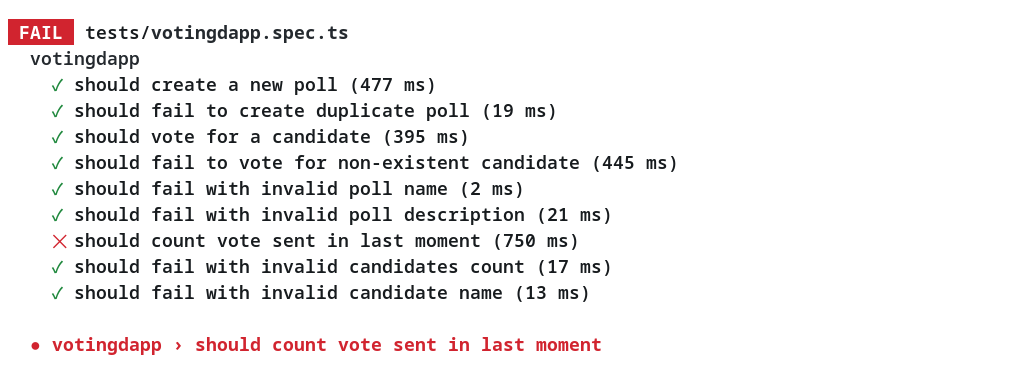
\includegraphics[width=\textwidth]{FuncTests}
    \caption{Результати функціонального тестування}
    \label{fig:functests}
  \end{figure}
  
  \subsubsection*{Підсумок тестування}
  
  За результатами проведеного функціонального тестування було виявлено, що з 9 запланованих тестових сценаріїв 8 було успішно виконано. Це свідчить про частковий успіх функціонального тестування із показником 89\% успішності.
  
  \subsubsection*{Відомі дефекти}

  \paragraph{Дефект:} Як описано в тестовому сценарії №5.1 --- якщо користувач подасть голос за гранично можливий час до завершення голосування --- голос не було зараховано.

  \paragraph{Причина:} Проблема полягає в недостатній кількості часу для передачі даних та успішного оброблення транзакції. Мережеві затримки, навантаження на мережу, час обробки транзакцій, а також внутрішня робота в застосунку займають час, протягом якого транзакція не може бути завершена.

  \paragraph{Статус:} дефект задокументовано, рішення недоцільне оскільки граничний час до завершення голосування протягом якого проявляється дефект є малим (менше 10мс) та не буде впливати на користувачів, що подають голос заздалегідь.
  
  \subsection{Тестування безпеки}
  
  \subsubsection*{Результат тестування}
  
  Результати тестування безпеки наведено в Додатку~\ref{app:sectests}. На рисунку~\ref{fig:sectests} зображено результати тестування безпеки застосунку.

  \begin{figure}[H]
    \centering
    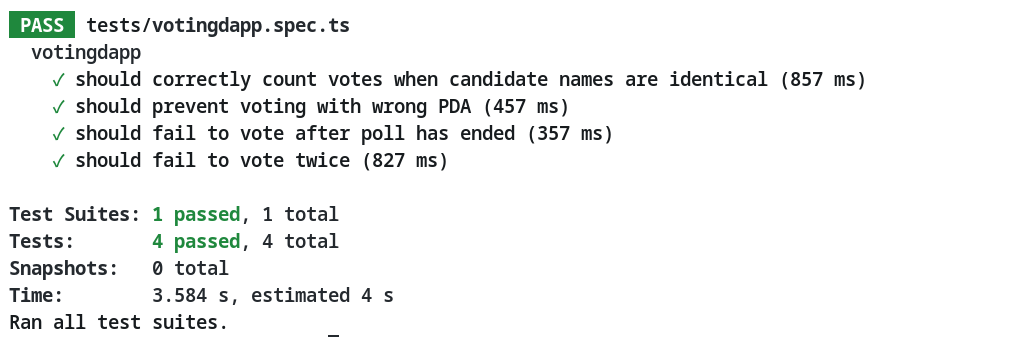
\includegraphics[width=\textwidth]{SecTests}
    \caption{Результати безпекового тестування}
    \label{fig:sectests}
  \end{figure}
  
  \subsubsection*{Підсумок тестування}
  
    За результатами проведеного безпекового тестування було виявлено, що всі 4 заплановані тестові сценарії було успішно виконано. Це свідчить про успіх безпекового тестування із показником 100\% успішності.
  
  \subsection{Тестування графічного інтерфейсу}
  
  \subsubsection*{Результат тестування}
  
  Результати тестування графічного інтерфейсу наведено в Додатку~\ref{app:guitests}. На рисунку~\ref{fig:guitests} зображено результати тестування графічного інтерфейсу застосунку.

  \begin{figure}[H]
    \centering
    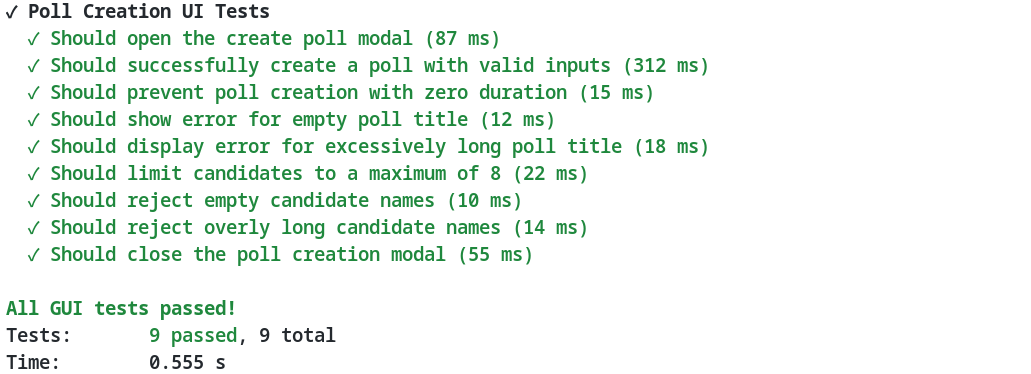
\includegraphics[width=\textwidth]{GuiTests}
    \caption{Результати тестування графічного інтерфейсу}
    \label{fig:guitests}
  \end{figure}
  
  \subsubsection*{Підсумок тестування}
  
  За результатами проведеного тестування графічного інтерфейсу було виявлено, що всі 9 запланованих тестових сценаріїв було успішно виконано. Це свідчить про успіх тестування графічного інтерфейсу із показником 100\% успішності.
  
  \subsection{Тестування продуктивності}
  
  \subsubsection*{Результат тестування}
  
  \subsubsection*{Підсумок тестування}
  
  \subsection{Метрики}
  
  
  \subsection{Критерій прийняття/відхилення релізу}
  
  
  \section{Висновки до розділу}
  
  % Розділ з економіки
  \tocnumchap{Економічна частина}
  
  \section{Економічна характеристика проєктного рішення}
  
  Метою роботи є розроблення застосунку для проведення голосувань з використанням технології блокчейну, що буде забезпечувати прозорість, незмінність результатів та виключати можливість фальсифікацій, що особливо важливо в умовах недовіри до традиційних способів голосування. Економічна доцільність проєкту полягає у зниженні витрат на організацію голосувань за рахунок автоматизації процесів, виключення паперових носіїв та мінімізації людського фактору. Система також не потребує додаткових витрат на перевірку достовірності результатів, оскільки дані зберігаються у захищеному блокчейні. Маркетингова оцінка свідчить про високу актуальність продукту: потенційними користувачами можуть бути державні органи, громадські організації, бізнес та освітні заклади. Завдяки прозорості, безпеці, гнучкості налаштувань і зручному інтерфейсу система має конкурентні переваги та перспективи комерціалізації через платну підписку або ліцензування.
  
  \section{Інформаційне забезпечення та формування гіпотези щодо потреби розроблення товару}
  
  Сфера децентралізованих технологій стрімко зростає, і водночас зростає суспільний запит на прозорі, захищені та недорогі способи прийняття колективних рішень. Існуючі системи голосування охоплюють централізовані офлайн-моделі з електронними урнами та сканерами, а також вебзастосунки для дистанційної участі, які мають обмеження у прозорості, довірі та безпеці. У свою чергу, децентралізовані рішення на базі блокчейн-технологій, як Voatz, пропонують підвищену прозорість і незмінність даних, хоча стикаються з викликами відкритості коду та аудиту. Водночас система i-Voting в Естонії, хоча і не базується на блокчейні, демонструє ефективність електронної ідентифікації та шифрування у масштабах держави. Основними споживачами запропонованої системи є організатори опитувань, локальні спільноти, державні установи та проєкти, що потребують прозорості і довіри. Аналіз ринку та конкурентів підтверджує необхідність створення нової системи на основі блокчейну Solana, яка поєднує зручність, безпеку та інноваційні функції.
  
  \section{Оцінювання та аналізування факторів зовнішнього та внутрішнього середовищ}
  
  Для оцінки доцільності розроблення запропонованого продукту доцільно розглянути та проаналізувати ключові фактори зовнішнього та внутрішнього середовищ, які впливають на перспективи впровадження системи. Нижче наведено результати експертного оцінювання впливу цих факторів, що дозволяють зробити комплексну оцінку умов для реалізації проєкту.
  
  \begin{tight}
  \begin{longtable}{|L{0.25}|C{0.2}|C{0.2}|C{0.2}|}
    \caption{\vspace{0.35em}\\\centering\textbf{Результати експертного оцінювання впливу факторів зовнішнього та внутрішнього середовищ}}
    \label{tab:ek1}\\\hline
    \multicolumn{1}{|c|}{\textbf{Фактори}} & \textbf{Середня експертна оцінка, бали} & \textbf{Середня вагомість факторів} & \textbf{Зважений рівень впливу, бали} \\\hline
    \multicolumn{1}{|c|}{\textbf{1}} & \textbf{2} & \textbf{3} & \textbf{4} \\\endfirsthead
    \multicolumn{4}{r}{Продовження табл. \thetable\vspace{0.35em}} \\\endhead\hline
    \multicolumn{4}{|c|}{\textit{Фактори зовнішнього середовища}} \\\hline
    Споживачі & 4 & 0,11 & 0,44 \\\hline
    Постачальники & 1 & 0,10 & 0,10 \\\hline
    Конкуренти & -2 & 0,10 & -0,20 \\\hline
    Державні органи влади & -1 & 0,05 & -0,05 \\\hline
    Інфраструктура & 2 & 0,06 & 0,12 \\\hline
    Законодавчі акти & -2 & 0,10 & -0,20 \\\hline
    Профспілки, партії та інші громадські організації & 0 & 0,05 & 0,00 \\\hline
    Система економічних відносин в державі & 1 & 0,06 & 0,06 \\\hline
    Організації-сусіди & 1 & 0,01 & 0,01 \\\hline
    Міжнародні події & 0 & 0,01 & 0,00 \\\hline
    Міжнародне оточення & 0 & 0,03 & 0,00 \\\hline
    Науково-технічний прогрес & 3 & 0,07 & 0,21 \\\hline
    Політичні обставини & -1 & 0,06 & -0,06 \\\hline
    Соціально-культурні обставини & 1 & 0,05 & 0,05 \\\hline
    Рівень техніки та технологій & 3 & 0,04 & 0,12 \\\hline
    Особливості міжнародних економічних відносин & 0 & 0,02 & 0,00 \\\hline
    Стан економіки & -1 & 0,08 & -0,08 \\\hline
    \multicolumn{2}{|c|}{\textbf{Загальна сума}} & \textbf{1} & \textbf{1,62} \\\hline
    \multicolumn{4}{|c|}{\textit{Фактори внутрішнього середовища}} \\\hline
    Цілі & 4 & 0,11 & 0,44 \\\hline
    Структура & 3 & 0,16 & 0,48 \\\hline
    Завдання & 3 & 0,07 & 0,21 \\\hline
    Технологія & 4 & 0,20 & 0,80 \\\hline
    Працівники & 4 & 0,21 & 0,84 \\\hline
    Ресурси & 3 & 0,25 & 0,75 \\\hline
    \multicolumn{2}{|c|}{\textbf{Загальна сума}} & \textbf{1} & \textbf{3,52} \\\hline
  \end{longtable}
  \end{tight}
  
  Проаналізувавши наведені дані, можна відзначити, що серед зовнішніх факторів найбільше позитивного впливу на діяльність системи надають споживачі, науково-технічний прогрес та рівень розвитку технологій. Водночас конкуренти, чинне законодавство та економічна ситуація створюють певні перешкоди. Що стосується внутрішніх чинників, найкраще оцінені працівники, технологічна база та доступні ресурси, що свідчить про високий потенціал для реалізації проєкту. Таким чином, результати експертної оцінки свідчать про наявність необхідності у розробці продукту та сприятливі умови для його виходу на ринок, що підтверджує обґрунтованість вибору напрямку для дипломної роботи.
  
  \section{Формування стратегічних альтернатив}
  
  Для програми обрано стратегію розвитку нового продукту, оскільки вона дозволяє створити унікальне програмне забезпечення, здатне задовольнити нові потреби користувачів та ринку. Враховуючи, що існуючі рішення не повністю відповідають сучасним вимогам, розроблення нового продукту відкриває можливості для інновацій та забезпечує конкурентні переваги. Такий підхід також передбачає потенційне розширення функціональності через супутні послуги, що підвищує цінність рішення для кінцевих споживачів.
  
  \section{Бюджетування}
    
  У таблиці \ref{tab:ek2} наведено бюджет витрат на матеріали та комплектуючі.  
  
  \begin{tight}
  \begin{longtable}{|C{0.25}|C{0.15}|C{0.1}|C{0.166}|C{0.16}|}
    \caption{\\\centering\textbf{Бюджет витрат матеріалів та комплектуючих виробів}}
    \label{tab:ek2}\\\hline
    \textbf{Назва матеріалів та комплектуючих} & \textbf{Марка, тип, модель} & \textbf{Кіль-кість, шт.} & \textbf{Ціна за одиницю, грн.} & \textbf{Разом, грн.} \\\hline\endfirsthead
    \multicolumn{5}{r}{Продовження табл. \thetable} \\\endhead\hline
    Зовнішній SSD-диск для зберігання резервних копій & Samsung T7 Shield 1TB USB 3.2 & 1 & 3\,400.00 & 3\,400.00 \\\hline
    Набір канцелярії & A4, ручки, стікери & 1 комплект & 300.00 & 300.00 \\\hline
    \textbf{Разом} &&& & \textbf{3\,700.00} \\\hline
  \end{longtable}
  \end{tight}

  У таблиці \ref{tab:ek3} показано бюджет на купівлю основних засобів, де вказані кількість одиниць, ціна, термін експлуатації амортизація.

  \begin{tight}
  \begin{longtable}{|C{0.12}|C{0.12}|C{0.095}|C{0.12}|C{0.12}|C{0.09}|C{0.11}|}
    \caption{\\\centering\textbf{Бюджет витрат на купівлю основних засобів}}
    \label{tab:ek3}\\\hline
    \textbf{Витрати на куповані засоби} & \textbf{Марка, тип, модель} & \textbf{Кіль-кість, шт.} & \textbf{Ціна за одиницю, грн.} & \textbf{Разом, грн.} & \textbf{Термін експлуатації, років} & \textbf{Місячна сума амортизації, грн.} \\\hline
    Ноутбук розробника & ASUS Vivobook Pro 15 OLED & 3 & 20\,000.00 & 60\,000.00 & 4 & 1\,250.00 \\\hline
    Смартфон для тестування мобільного застосунку & Samsung Galaxy A34 5G 6/128GB & 1 & 10\,500.00 & 10\,500.00 & 3 & 291.67 \\\hline
    Монітор зовнішній & LG 24MP60G-B 24” IPS FHD & 1 & 5\,000.00 & 5\,000.00 & 5 & 83.33 \\\hline
    \multicolumn{4}{|c|}{\textbf{Разом}} & \textbf{75\,500.00} & & \textbf{1\,625.00} \\\hline
  \end{longtable}
  \end{tight}
  
  Таблиця \ref{tab:ek4} містить бюджет витрат на оплату праці, розділений на основну зарплату та додаткову (премії 10\%), враховано кількість працівників і робочі дні.
  
  \begin{tight}
  \begin{longtable}{|C{0.2}|C{0.15}|C{0.15}|C{0.166}|C{0.16}|}
    \caption{\vspace{0.35em}\\\centering\textbf{Бюджет витрат на оплату праці}}
    \label{tab:ek4}\\\hline
    \textbf{Посада, спеціальність} & \textbf{Кількість працівників, осіб} & \textbf{Час роботи, дні} & \textbf{Денна заробітна плата працівників, грн.} & \textbf{Сума витрат на оплату праці, грн.} \\\hline\endfirsthead
    \multicolumn{5}{r}{Продовження табл. \thetable\vspace{0.35em}} \\\endhead\hline
    \multicolumn{5}{|c|}{\textit{Основна заробітна плата}} \\\hline
    Керівник проєкту & 1 & 22 & 1\,000.00 & 22\,000.00 \\\hline
    Розробник ПЗ & 1 & 10 & 2\,000.00 & 20\,000.00 \\\hline
    Менеджер зі збуту & 1 & 22 & 1\,000.00 & 22\,000.00 \\\hline
    \multicolumn{4}{|c|}{\textbf{Разом}} & \textbf{64\,000} \\\hline
    \multicolumn{5}{|c|}{\textit{Додаткова заробітна плата (премії, надбавки)}} \\\hline
    Премія керівнику (10\%) & 1 & – & – & 2\,200.00 \\\hline
    Премія розробнику (10\%) & 1 & – & – & 2\,000.00 \\\hline
    Премія менеджеру зі збуту (10\%) & 1 & – & – & 2\,200.00 \\\hline
    \multicolumn{4}{|c|}{\textbf{Разом}} & \textbf{6\,400.00} \\\hline
  \end{longtable}
  \end{tight}

  В таблиці \ref{tab:ek5} наведено розрахунок обов’язкових відрахувань і податків, зокрема єдиного внеску на соціальне страхування, який становить 22\% від зарплати.

  \begin{tight}
  \begin{longtable}{|C{0.2}|C{0.15}|C{0.15}|C{0.166}|C{0.16}|}
    \caption{\vspace{0.35em}\\\centering\textbf{Бюджет обов'язкових відрахувань та податків}}
    \label{tab:ek5}\\\hline
    \textbf{Посада, спеціальність} & \textbf{Сума основної заробітної плати} & \textbf{Сума додаткової заробітної плати} & \textbf{Разом витрат на оплату праці} & \textbf{Сума єдиного внеску на соціальне страхування, грн.} \\\hline\endfirsthead
    \multicolumn{5}{r}{Продовження табл. \thetable\vspace{0.35em}} \\\endhead\hline
    Керівник проєкту & 22\,000.00 & 2\,200.00 & 24\,200.00 & 5\,324.00 \\\hline
    Розробник ПЗ & 20\,000.00 & 2\,000.00 & 22\,000.00 & 4\,840.00 \\\hline
    Менеджер зі збуту & 22\,000.00 & 2\,200.00 & 24\,200.00 & 5\,324.00 \\\hline
    \multicolumn{3}{|c|}{\textbf{Разом}} & \textbf{70\,400.00} & \textbf{15\,488.00} \\\hline
  \end{longtable}
  \end{tight}

  У таблиці \ref{tab:ek6} представлено бюджет загальновиробничих витрат, що включає змінні й постійні складові; додаткові витрати на допоміжний персонал та інші статті не передбачені, оскільки всі необхідні функції забезпечуються вже залученими працівниками без потреби у додаткових ресурсах.

  \begin{tight}
  \begin{longtable}{|L{0.6}|C{0.3}|}
    \caption{\vspace{0.35em}\\\centering\textbf{Бюджет загальновиробничих витрат}}
    \label{tab:ek6}\\\hline
    \multicolumn{1}{|c|}{\textbf{Статті витрат}} & \textbf{Сума, грн.} \\\hline\endfirsthead
    \multicolumn{2}{r}{Продовження табл. \thetable\vspace{0.35em}} \\\endhead\hline
    \multicolumn{2}{|c|}{\textit{Змінні загальновиробничі витрати}} \\\hline
    Заробітна плата допоміжного персоналу & 0.00 \\ \hline
    Витрати на МШП & 3\,700.00 \\ \hline
    Витрати на електроенергію та технологічні цілі & 1\,000.00 \\ \hline
    Витрати на ремонт & 0.00 \\ \hline
    Інші змінні витрати & 0.00 \\ \hline
    \textbf{Разом змінних витрат} & \textbf{4\,700.00} \\\hline
    \multicolumn{2}{|c|}{\textit{Постійні загальновиробничі витрати}} \\\hline
    Заробітна плата допоміжного персоналу & 0.00 \\ \hline
    Комунальні послуги & 1\,000.00 \\ \hline
    Витрати на оренду & 10\,000.00 \\ \hline
    Витрати на ремонт & 0.00 \\ \hline
    Інші постійні витрати & 0.00 \\ \hline
    Разом постійних витрат & 11\,000.00 \\\hline
    \textbf{Разом загальновиробничих витрат} & \textbf{15\,700.00} \\\hline
  \end{longtable}
  \end{tight}
  
  Таблиця \ref{tab:ek7} містить дані про адміністративні витрати та витрати на збут.
  
  \begin{tight}
  \begin{longtable}{|L{0.6}|C{0.3}|}
    \caption{\vspace{0.35em}\\\centering\textbf{Бюджет адміністративних витрат та витрат на збут}}
    \label{tab:ek7}\\\hline
    \multicolumn{1}{|c|}{\textbf{Статті витрат}} & \textbf{Сума, грн.} \\\hline
    \multicolumn{1}{|c|}{\textbf{1}} & \textbf{2} \\\endfirsthead
    \multicolumn{2}{r}{Продовження табл. \thetable\vspace{0.35em}} \\\endhead\hline
    \multicolumn{2}{|c|}{\textit{Адміністративні витрати}} \\ \hline
    Заробітна плата адміністративного персоналу & 22\,000.00\\ \hline
    Витрати на МШП & 3\,700.00 \\ \hline
    Витрати на відрядження & 0.00 \\ \hline
    Витрати на ремонт & 0.00 \\ \hline
    Витрати на паливно-мастильні матеріали & 0.00 \\ \hline
    Витрати на сплату податків і зборів & 4\,840.00 \\ \hline
    Знос адміністративного обладнання & 0.00\\ \hline
    \textbf{Разом адміністративних витрат} & \textbf{30\,540.00}\\ \hline
    \multicolumn{2}{|c|}{\textit{Витрати на збут}} \\ \hline
    Заробітна плата менеджерів зі збуту & 22\,000.00\\ \hline
    Витрати на гарантійний ремонт & 0.00 \\ \hline
    Витрати на відрядження & 0.00 \\ \hline
    Витрати на гарантійне обслуговування & 10\,000.00 \\ \hline
    Витрати на налагодження і експлуатацію & 10\,000.00 \\ \hline
    Витрати на паливно-мастильні матеріали & 0.00 \\ \hline
    Витрати на сплату податків і зборів & 4\,840.00 \\ \hline
    Витрати на рекламу & 40\,000.00\\ \hline
    \textbf{Разом витрат на збут} & \textbf{86\,840.00}\\ \hline
  \end{longtable}
  \end{tight}
  
  У таблиці \ref{tab:ek8} підсумовано всі основні витрати на розробку проєкту, утворюючи зведений кошторис. Витрати на сировину і матеріали та зворотні відходи не передбачені.
  
  \vspace{-1em}
  
  \begin{tight}
  \begin{longtable}{|L{0.6}|C{0.3}|}
    \caption{\vspace{0.35em}\\\centering\textbf{Зведений кошторис витрат на розробку проєктного рішення (продукту)}}
    \label{tab:ek8}\\\hline
    \multicolumn{1}{|c|}{\textbf{Статті витрат}} & \textbf{Разом, грн.} \\\hline\endfirsthead
    \multicolumn{2}{r}{Продовження табл. \thetable\vspace{0.35em}} \\\endhead\hline
    Купівельні напівфабрикати та комплектуючі вироби & 3\,700.00 \\\hline
    Паливо та електроенергія на технологічні цілі & 1\,000.00 \\\hline
    Амортизаційні відрахування основних фондів & 1\,625.00\\\hline
    Основна заробітна плата & 64\,000.00 \\\hline
    Додаткова заробітна плата & 6\,400.00 \\\hline
    Відрахування на соціальне страхування & 15\,488.00 \\\hline
    Витрати на утримання й експлуатацію устаткування & 0.00 \\\hline
    Змінні загальновиробничі витрати & 4\,700.00 \\\hline
    Постійні загальновиробничі витрати & 11\,000.00 \\\hline
    \textbf{Разом загальновиробничих витрат} & \textbf{107\,913.00}\\\hline
    Адміністративні витрати & 30\,540.00 \\\hline
    Витрати на збут & 86\,840.00 \\\hline
    Інші операційні витрати & 0.00 \\\hline
    \textbf{Разом виробничих і операційних витрат} & \textbf{225\,293.00} \\\hline
  \end{longtable}
  \end{tight}
  
  В таблиці \ref{tab:ek9} наведено розрахунок собівартості продукції і планованої ціни продажу з урахуванням рентабельності 30\% при обсязі продажу 5 одиниць.
  
  \begin{tight}
  \begin{longtable}{|L{0.6}|C{0.3}|}
    \caption{\vspace{0.35em}\\\centering\textbf{Бюджет фінансових результатів}}
    \label{tab:ek9}\\
    \hline
    \multicolumn{1}{|c|}{\textbf{Показники}} & \textbf{Сума, грн.} \\\hline
    \multicolumn{1}{|c|}{\textbf{1}} & \textbf{2} \\\endfirsthead
    \multicolumn{2}{r}{Продовження табл. \thetable\vspace{0.35em}} \\\endhead\hline
    Дохід від реалізації продукції & 701\,434.50 \\\hline
    Податок на додану вартість & 140\,286.90 \\\hline
    Чистий дохід від реалізації продукції & 561\,147.60 \\\hline
    Собівартість реалізованої продукції & 107\,913.00 \\\hline
    Валовий прибуток & 453\,234.60 \\\hline
    Адміністративні витрати & 30\,540.00 \\\hline
    Витрати на збут & 86\,840.00 \\\hline
    Інші операційні витрати & 0.00 \\\hline
    Фінансовий результат від операційної діяльності & 335\,854.60 \\\hline
    Податок на прибуток & 60\,453.83 \\\hline
    Чистий прибуток (збиток) & 275\,400.77 \\\hline
  \end{longtable}
  \end{tight}
  
  \section{Висновки до розділу}
  
  У роботі проведено аналіз ринку, середовища, стратегічних альтернатив та економічного обґрунтування, що дозволило сформувати чітке уявлення про перспективи впровадження програмного забезпечення. Враховано основні характеристики продукту, його технічні специфікації та вигоди для кінцевих користувачів, що забезпечує конкурентні переваги на ринку.

  Обрана стратегія — стратегія нового продукту, що передбачає впровадження інноваційного рішення з унікальними властивостями. Такий підхід відповідає ринковим тенденціям і дозволяє максимально задовольнити потреби цільової аудиторії.

  Ціна програмного забезпечення становить 140\,286.90 грн. За прогнозом, реалізація обраної стратегії забезпечить чистий прибуток у розмірі 275\,400.77 грн, що свідчить про економічну ефективність проєкту та його перспективність для інвесторів.
  
  \tocchap{Висновки}
  
  \renewcommand\bibname{\MakeUppercase{Список літератури}}
  \addcontentsline{toc}{chapter}{\MakeUppercase{Список літератури}}
  \begin{thebibliography}{99}
    \bibitem{blockchain_structure} Blockchain structure. URL: \url{https://www.researchgate.net/publication/369352496/figure/fig1/AS:11431281414772432@1746017302739/Blockchain-structure.tif}.

    (дата звернення 13.05.2025)
    \bibitem{blockchain} Awosika E. What Is Blockchain Voting?. URL: \url{https://second-pocket-shoot-73.hashnode.dev/what-is-blockchain-voting}.

    (дата звернення 22.01.2025)
    \bibitem{consensus} PoH, PoS, PoW - Explained. \textit{Helius}. URL: \url{https://www.helius.dev/blog/proof-of-history-proof-of-stake-proof-of-work-explained}.
    
    (дата звернення 22.01.2025)
    \bibitem{pow} Porat, A., Pratap, A., Shah, P. Blockchain Consensus: An analysis of Proof-of-Work and its applications. \textit{Stanford University}. URL: \url{https://www.scs.stanford.edu/17au-cs244b/labs/projects/porat_pratap_shah_adkar.pdf}.
    
    (дата звернення 22.01.2025)
    \bibitem{pos} C. T. Nguyen, D. T. Hoang, D. N. Nguyen. Proof-of-Stake Consensus Mechanisms for Future Blockchain Networks: Fundamentals, Applications and Opportunities. \textit{IEEE Access}. 2019. Ст. 5-9. DOI: 10.1109/ACCESS.2019.2925010.
    \bibitem{poh} Victor S. Proof of history: what is it good for? URL: \url{https://www.shoup.net/papers/poh.pdf}.
    
    (дата звернення 22.01.2025)
    \bibitem{voatz} Security and technology. \textit{Voatz}. URL: \url{https://voatz.com/security-and-technology/}.
    
    (дата звернення 22.01.2025)
    \bibitem{voatzcriticism} Specter M. A., Koppel J., Weitzner D. The Ballot is Busted Before the Blockchain: A Security Analysis of Voatz, the First Internet Voting Application Used in U.S. Federal Elections. \textit{MIT}. URL: \url{https://internetpolicy.mit.edu/wp-content/uploads/2020/02/SecurityAnalysisOfVoatz_Public.pdf}.

    (дата звернення 13.05.2025)
    \bibitem{ivoting} Introduction to i-voting. \textit{Valimised}. 
    URL: \url{https://www.valimised.ee/en/internet-voting/more-about-i-voting/introduction-i-voting}.
    
    (дата звернення 17.01.2025)
    \bibitem {ieee:almeida} Almeida, R. L., Baiardi, F., Maesa, D. D. F., \& Ricci, L. Impact of Decentralization on Electronic Voting Systems: A Systematic Literature Survey. \textit{IEEE Access}. 2023. Ст. 31. DOI: 10.1109/ACCESS.2023.3336593.
    \bibitem{solana_report} Network Performance Report - October 2022. \textit{Solana}. URL: \url{https://solana.com/news/network-performance-report-october-2022}.
    
    (дата звернення 18.03.2025)
  \end{thebibliography}
  
  \appendix
  \renewcommand{\thechapter}{\Alph{chapter}}
  \renewcommand{\chaptername}{Додаток}
 
  \tocnumchap{Приклад інтерфейсу користувача}
  \label{app:UI}
  
  \begin{figure}[H]
    \centering
    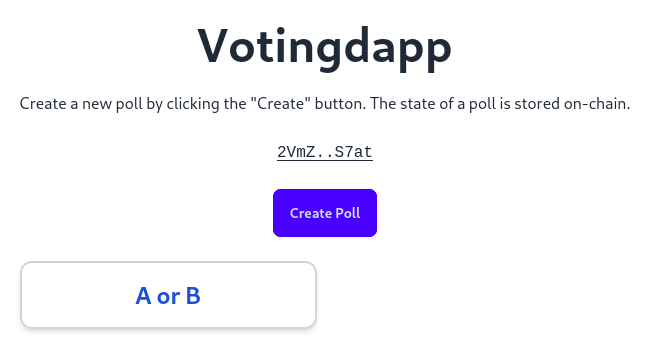
\includegraphics[scale=0.2]{UIPolls}
    \caption{Перегляд списку голосувань}
    \label{fig:UIPolls}
  \end{figure}
  
  \begin{figure}[H]
    \centering
    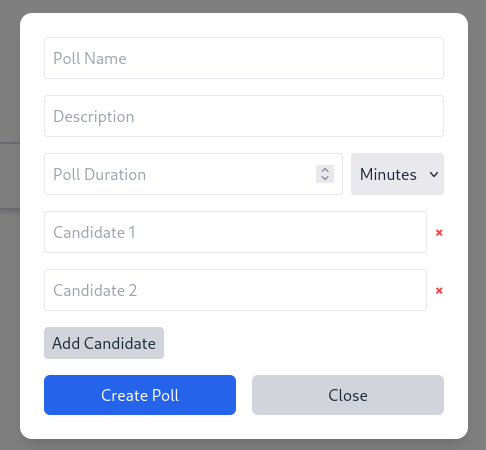
\includegraphics[scale=0.5]{UICreate}
    \caption{Форма для створення голосування}
    \label{fig:UICreate}
  \end{figure}
  
  \begin{figure}[H]
    \centering
    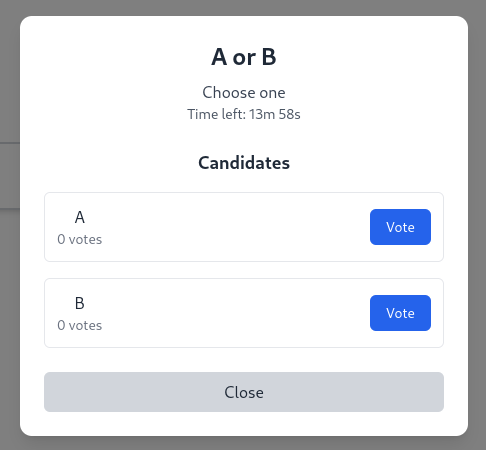
\includegraphics[scale=0.5]{UIVote}
    \caption{Форма для подачі голосу}
    \label{fig:UIVote}
  \end{figure}
  
  \begin{figure}[H]
    \centering
    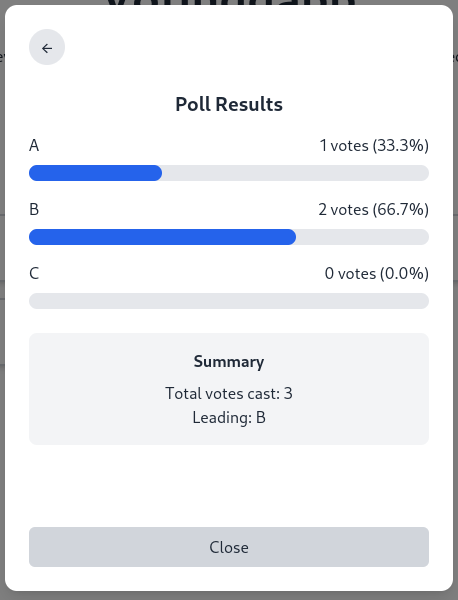
\includegraphics[scale=0.5]{UIResults}
    \caption{Перегляд результатів голосування}
    \label{fig:UIResults}
  \end{figure}
  
  \begin{figure}[H]
    \centering
    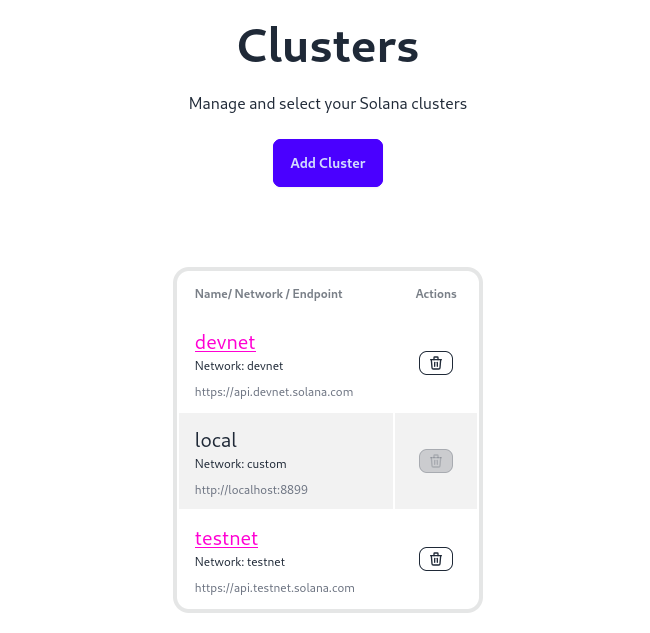
\includegraphics[scale=0.5]{UIClusters}
    \caption{Сторінка зі списком кластерів мережі}
    \label{fig:UIClusters}
  \end{figure}
  
  \begin{figure}[H]
    \centering
    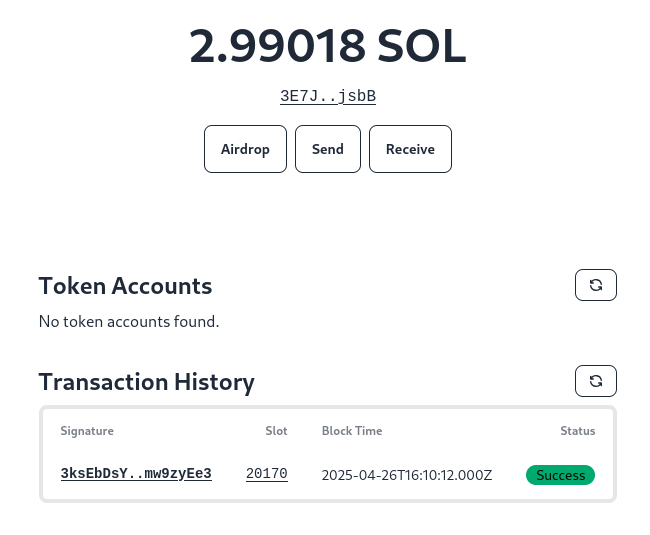
\includegraphics[scale=0.5]{UIAccount}
    \caption{Відображення інформації про баланс акаунту та історії транзакцій}
    \label{fig:UIAccount}
  \end{figure}
  
  \tocnumchap{Інструкція користувача}
  \label{app:instruction}
  
  \section*{Компоненти ПЗ}
  
  Розроблене програмне забезпечення реалізовано з використанням мови програмування Rust. Як середовище розробки застосовано редактор коду Helix та термінал fish. Було використано систему керування пакетами Cargo для збирання проєкту, а також бібліотеки, пов’язані із взаємодією з блокчейн-платформою Solana. Серверна логіка реалізована як смарт-контракт, який виконується на блокчейні, а клієнтська частина – у вигляді React-застосунку.

  Програмне забезпечення потребує мінімальні апаратні ресурси. Достатньо персонального комп’ютера з двоядерним процесором, 4 ГБ оперативної пам’яті, встановленою ОС на базі Linux, macOS або Windows та доступом до інтернету. Для роботи потрібна попередньо встановлена Solana CLI (версія 2.1.17), Anchor CLI (версія 0.30.1), Rust toolchain (версія 1.83.0) та Node.js ( версія 22.14.0). Список основних файлів проєкту необхідних для розгортання застосунку із поясненням їхнього призначення наведено в таблиці \ref{tab:instr1}.

  \begin{tight}
  \begin{longtable}{|C{0.03}|C{0.3}|L{0.5}|}
    \caption{\vspace{0.35em}\\\centering\textbf{Основні файли проєкту}}
    \label{tab:instr1}\\\hline
    \textbf{№} & \textbf{Файл} & \multicolumn{1}{|c|}{\textbf{Призначення}} \\\hline\endfirsthead
    \multicolumn{3}{r}{Продовження табл. \thetable\vspace{0.35em}} \\\hline
    \textbf{№} & \textbf{Файл} & \multicolumn{1}{|c|}{\textbf{Призначення}} \\\hline\endhead\hline
    1 & anchor/Anchor.toml & Файл конфігурації Anchor, що містить налаштування проєкту, адреси програм, параметри середовища та кластерів для розгортання. \\\hline
    2 & anchor/target/idl/*.json & Опис інтерфейсу смарт-контракту у форматі JSON, який використовується для взаємодії клієнтської частини з програмою. \\\hline
    3 & anchor/target/deploy/*.so & Скомпільований байткод смарт-контракту, готовий для розгортання в мережі Solana. \\\hline
    4 & keypair.json & Файл із закритим ключем програми, необхідний для розгортання смарт-контракту. \\\hline
  \end{longtable}
  \end{tight}
  
  \section*{Встановлення ПЗ}
  
  Для встановлення застосунку необхідно мати встановлені Solana CLI (версія 2.1.17), Anchor CLI (версія 0.30.1) та Node.js (версія 22.14.0).  

  Перед розгортанням смарт-контракту потрібно згенерувати файл з парою ключів програми \texttt{keypair.json} і вказати його шлях у \texttt{anchor/Anchor.toml}.

  Для розгортання смарт-контракту слід задати адресу потрібного кластера Solana у файлі \texttt{anchor/Anchor.toml}, після чого виконати команду \texttt{npm run anchor deploy}.
  
  Для розгортання клієнтської частини достатньо виконати команду \texttt{npm install \&\& npm run build \&\& npm start}.
  
  \section*{Налаштування ПЗ}
  
  Для коректної роботи програми необхідно налаштувати підключення до мережі Solana, вказати адресу кластера, а також забезпечити наявність достатнього балансу SOL на акаунті користувача. Крім того, слід правильно розгорнути смарт-контракт.
  
  \section*{Базові функції ПЗ}
  
  Розроблене програмне забезпечення дозволяє створювати та проводити голосування на базі блокчейну Solana. Один зі способів доступу до функцій — через клієнтський веб-інтерфейс, який забезпечує взаємодію користувача з системою.
  
  \section*{Аналіз помилок}
  
  Якщо клієнтський інтерфейс відображає помилку доступу до програми, необхідно впевнитися в успішному розгортанні смарт-контракту.
  
  Якщо клієнтський інтерфейс відображає помилку підключення до кластера Solana, необхідно перевірити стабільність інтернет-з’єднання та доступність самого кластера.
  
  Якщо на балансі акаунту недостатньо SOL, потрібно скористатися функцією airdrop для поповнення балансу.
  
  \tocnumchap{Програмний код}
  \label{app:code}
  
  \begin{multicols}{2}
  
  \textbf{Файл anchor/Anchor.toml}
  {\lstset{basicstyle=\fontsize{8}{10}\selectfont\ttfamily}
  \lstinputlisting{~/Repositories/voting-dapp/anchor/Anchor.toml}
  }

  \end{multicols}
  
  \tocnumchap{Тестові випадки функціональних тестів}
  \label{app:functests}
  
  \begin{tight}
  \begin{longtable}{|C{0.5}|C{0.2}|C{0.175}|}
    \caption{\vspace{0.35em}\\\centering\textbf{Тестові випадки функціональних тестів}}
    \label{tab:functests}\\\hline
    \textbf{ID | Name} & \multicolumn{2}{|c|}{\textbf{Опис}} \\\hline\endfirsthead
    \multicolumn{3}{r}{Продовження табл. \thetable\vspace{0.35em}} \\\hline\endhead\hline
    
    №1.1 | Створення опитування & \multicolumn{2}{|L{0.375}|}{Перевірка успішного створення нового опитування} \\\hline
    \textbf{Кроки} & \textbf{Очікування} & \textbf{Результат} \\\hline
    \begin{enumerate}
      \item Викликати метод createPoll
      \item Вказати коректні параметри
    \end{enumerate} & 
    Опитування створено з правильними даними
    & Passed \\\hline

    №1.2 | Дублювання опитування & \multicolumn{2}{|L{0.375}|}{Спроба створити опитування з існуючою назвою} \\\hline
    \textbf{Кроки} & \textbf{Очікування} & \textbf{Результат} \\\hline
    \begin{enumerate}
      \item Викликати метод createPoll
      \item Використати існуючу назву опитування
    \end{enumerate} & 
    Помилка "Poll already exists"
    & Passed \\\hline
    
    №2.1 | Голосування & \multicolumn{2}{|L{0.375}|}{Успішне голосування за кандидата} \\\hline
    \textbf{Кроки} & \textbf{Очікування} & \textbf{Результат} \\\hline
    \begin{enumerate}
      \item Викликати метод vote
      \item Вказати існуючого кандидата
    \end{enumerate} & 
    Кількість голосів збільшена на 1
    & Passed \\\hline

    №2.2 | Голосування за неіснуючого кандидата & \multicolumn{2}{|L{0.375}|}{Спроба проголосувати за неіснуючого кандидата} \\\hline
    \textbf{Кроки} & \textbf{Очікування} & \textbf{Результат} \\\hline
    \begin{enumerate}
      \item Викликати метод vote
      \item Вказати неіснуюче ім'я кандидата
    \end{enumerate} & 
    Помилка "Candidate not found"
    & Passed \\\hline

    №3.1 | Некоректна назва опитування & \multicolumn{2}{|L{0.375}|}{Спроба створити опитування з надто довгою або порожньою назвою} \\\hline
    \textbf{Кроки} & \textbf{Очікування} & \textbf{Результат} \\\hline
    \begin{enumerate}
      \item Викликати метод createPoll
      \item Вказати порожню назву або довше 32 символів
    \end{enumerate} & 
    Помилка "Invalid poll name"
    & Passed \\\hline
    
    №3.2 | Некоректний опис опитування & \multicolumn{2}{|L{0.375}|}{Спроба створити опитування з надто довгим або порожнім описом} \\\hline
    \textbf{Кроки} & \textbf{Очікування} & \textbf{Результат} \\\hline
    \begin{enumerate}
      \item Викликати метод createPoll
      \item Вказати порожній опис або довше 64 символів
    \end{enumerate} & 
    Помилка "Invalid poll description"
    & Passed \\\hline
    
    №4.1 | Некоректна назва кандидата & \multicolumn{2}{|L{0.375}|}{Спроба створити кандидата з надто довгою або порожньою назвою} \\\hline
    \textbf{Кроки} & \textbf{Очікування} & \textbf{Результат} \\\hline
    \begin{enumerate}
      \item Викликати метод createPoll
      \item Вказати порожню назву кандидата або довше 32 символів
    \end{enumerate} & 
    Помилка "Invalid candidate name"
    & Passed \\\hline
    
    №4.2 | Некоректна кількість кандидатів & \multicolumn{2}{|L{0.375}|}{Спроба створити опитування з надто великою кількістю кандидатів} \\\hline
    \textbf{Кроки} & \textbf{Очікування} & \textbf{Результат} \\\hline
    \begin{enumerate}
      \item Викликати метод createPoll
      \item Вказати кандидатів, кількість яких більша 8
    \end{enumerate} & 
    Помилка "Invalid candidate count"
    & Passed \\\hline
    
    №5.1 | Голосування в останній момент перед завершенням & \multicolumn{2}{|L{0.375}|}{Спроба проголосувати в останній момент перед завершенням голосування} \\\hline
    \textbf{Кроки} & \textbf{Очікування} & \textbf{Результат} \\\hline
    \begin{enumerate}
      \item Створити опитування з часом до завершення
      \item Викликати метод vote за 10мс до завершення
    \end{enumerate} & 
    Успішне зарахування голосу
    & Failed \\\hline
  \end{longtable}
  \end{tight}
  
  \tocnumchap{Тестові випадки тестів безпеки}
  \label{app:sectests}
  
  \begin{tight}
  \begin{longtable}{|C{0.5}|C{0.2}|C{0.175}|}
    \caption{\vspace{0.35em}\\\centering\textbf{Тестові випадки тестів безпеки}}
    \label{tab:sectests}\\\hline
    \textbf{ID | Name} & \multicolumn{2}{|c|}{\textbf{Опис}} \\\hline\endfirsthead
    \multicolumn{3}{r}{Продовження табл. \thetable\vspace{0.35em}} \\\hline\endhead\hline
    
    №1.1 | Голосування з невірним \gls{pda} & \multicolumn{2}{|L{0.375}|}{Спроба проголосувати, використовуючи невірний \gls{pda}} \\\hline
    \textbf{Кроки} & \textbf{Очікування} & \textbf{Результат} \\\hline
    \begin{enumerate}
      \item Створити опитування
      \item Згенерувати некоректний \gls{pda} для виборця
      \item Викликати метод vote з некоректним \gls{pda}
    \end{enumerate} & 
    Транзакція відхилена; кількість голосів не змінюється
    & Passed \\\hline
    
    №2.1 | Повторне голосування & \multicolumn{2}{|L{0.375}|}{Спроба проголосувати вдруге} \\\hline
    \textbf{Кроки} & \textbf{Очікування} & \textbf{Результат} \\\hline
    \begin{enumerate}
      \item Викликати метод vote
      \item Використати той самий гаманець
    \end{enumerate} & 
    Помилка "Already voted"
    & Passed \\\hline
    
    №2.2 | Голосування після завершення & \multicolumn{2}{|L{0.375}|}{Спроба проголосувати у завершеному опитуванні} \\\hline
    \textbf{Кроки} & \textbf{Очікування} & \textbf{Результат} \\\hline
    \begin{enumerate}
      \item Створити опитування з коротким часом до завершення
      \item Зачекати завершення
      \item Викликати метод vote
    \end{enumerate} & 
    Помилка "Voting ended"
    & Passed \\\hline
    
    №3.1 | Неунікальні назви кандидатів & \multicolumn{2}{|L{0.375}|}{Спроба проголосувати в опитуванні з кандидатами, що мають однакові назви} \\\hline
    \textbf{Кроки} & \textbf{Очікування} & \textbf{Результат} \\\hline
    \begin{enumerate}
      \item Створити опитування з кандидатами з однаковими назвами
      \item Викликати метод vote для другого кандидата в списку
    \end{enumerate} & 
    Голос зараховується другому кандидату
    & Passed \\\hline
  \end{longtable}
  \end{tight}
  
  \tocnumchap{Тестові випадки тестів графічного інтерфейсу}
  \label{app:guitests}
  
  \begin{tight}
  \begin{longtable}{|C{0.5}|C{0.2}|C{0.175}|}
    \caption{\vspace{0.35em}\\\centering\textbf{Тестові випадки тестів графічного інтерфейсу}}
    \label{tab:guitests}\\\hline
    \textbf{ID | Name} & \multicolumn{2}{|c|}{\textbf{Опис}} \\\hline\endfirsthead
    \multicolumn{3}{r}{Продовження табл. \thetable\vspace{0.35em}} \\\hline\endhead\hline

    №1.1 | Відкриття модального вікна & \multicolumn{2}{|L{0.375}|}{Перевірка відкриття вікна створення опитування} \\\hline
    \textbf{Кроки} & \textbf{Очікування} & \textbf{Результат} \\\hline
    \begin{enumerate}
      \item Натиснути кнопку "Create Poll"
    \end{enumerate} &
    Відображається модальне вікно з формою опитування
    & Passed \\\hline

    №1.2 | Успішне створення опитування & \multicolumn{2}{|L{0.375}|}{Заповнення всіх полів коректними значеннями} \\\hline
    \textbf{Кроки} & \textbf{Очікування} & \textbf{Результат} \\\hline
    \begin{enumerate}
      \item Заповнити поля: назва, опис, 2 кандидати, тривалість = 10, одиниця = хвилини
      \item Натиснути кнопку створення
    \end{enumerate} &
    Опитування успішно створено, модальне вікно закрито
    & Passed \\\hline

    №1.3 | Некоректна тривалість & \multicolumn{2}{|L{0.375}|}{Спроба створити опитування з тривалістю = 0} \\\hline
    \textbf{Кроки} & \textbf{Очікування} & \textbf{Результат} \\\hline
    \begin{enumerate}
      \item Вказати тривалість = 0
      \item Натиснути кнопку створення
    \end{enumerate} &
    Повідомлення про помилку "Duration must be greater than 0"
    & Passed \\\hline

    №1.4 | Порожнє поле назви & \multicolumn{2}{|L{0.375}|}{Спроба створити опитування без назви} \\\hline
    \textbf{Кроки} & \textbf{Очікування} & \textbf{Результат} \\\hline
    \begin{enumerate}
      \item Очистити поле назви
      \item Натиснути кнопку створення
    \end{enumerate} &
    Повідомлення про помилку "Poll name is required"
    & Passed \\\hline

    №1.5 | Довга назва & \multicolumn{2}{|L{0.375}|}{Спроба ввести назву довжиною понад 64 байти} \\\hline
    \textbf{Кроки} & \textbf{Очікування} & \textbf{Результат} \\\hline
    \begin{enumerate}
      \item Ввести назву довжиною понад 64 символи
      \item Натиснути кнопку створення
    \end{enumerate} &
    Повідомлення про помилку "Poll name is too long"
    & Passed \\\hline

    №1.6 | Більше 8 кандидатів & \multicolumn{2}{|L{0.375}|}{Спроба додати більше 8 кандидатів} \\\hline
    \textbf{Кроки} & \textbf{Очікування} & \textbf{Результат} \\\hline
    \begin{enumerate}
      \item Додати 9 полів кандидатів
    \end{enumerate} &
    Повідомлення про помилку "Maximum 8 candidates allowed"
    & Passed \\\hline

    №1.7 | Порожнє поле кандидата & \multicolumn{2}{|L{0.375}|}{Один з кандидатів має порожню назву} \\\hline
    \textbf{Кроки} & \textbf{Очікування} & \textbf{Результат} \\\hline
    \begin{enumerate}
      \item Один з кандидатів має порожню назву
      \item Натиснути кнопку створення
    \end{enumerate} &
    Повідомлення про помилку "Candidate name can't be empty"
    & Passed \\\hline

    №1.8 | Довге ім’я кандидата & \multicolumn{2}{|L{0.375}|}{Спроба ввести назву кандидата понад 32 символи} \\\hline
    \textbf{Кроки} & \textbf{Очікування} & \textbf{Результат} \\\hline
    \begin{enumerate}
      \item Додати кандидата з назвою понад 32 символи
    \end{enumerate} &
    Повідомлення про помилку "Candidate name too long"
    & Passed \\\hline

    №1.9 | Закриття модального вікна & \multicolumn{2}{|L{0.375}|}{Перевірка закриття модального вікна} \\\hline
    \textbf{Кроки} & \textbf{Очікування} & \textbf{Результат} \\\hline
    \begin{enumerate}
      \item Натиснути кнопку "×" або "Cancel"
    \end{enumerate} &
    Модальне вікно закрите
    & Passed \\\hline
  \end{longtable}
  \end{tight}
  
\end{document}